\documentclass[chi_draft]{sigchi}

% Use this command to override the default ACM copyright statement
% (e.g. for preprints).  Consult the conference website for the
% camera-ready copyright statement.

%% EXAMPLE BEGIN -- HOW TO OVERRIDE THE DEFAULT COPYRIGHT STRIP -- (July 22, 2013 - Paul Baumann)
% \toappear{Permission to make digital or hard copies of all or part of this work for personal or classroom use is      granted without fee provided that copies are not made or distributed for profit or commercial advantage and that copies bear this notice and the full citation on the first page. Copyrights for components of this work owned by others than ACM must be honored. Abstracting with credit is permitted. To copy otherwise, or republish, to post on servers or to redistribute to lists, requires prior specific permission and/or a fee. Request permissions from permissions@acm.org. \\
% {\emph{CHI'14}}, April 26--May 1, 2014, Toronto, Canada. \\
% Copyright \copyright~2014 ACM ISBN/14/04...\$15.00. \\
% DOI string from ACM form confirmation}
%% EXAMPLE END -- HOW TO OVERRIDE THE DEFAULT COPYRIGHT STRIP -- (July 22, 2013 - Paul Baumann)

% Arabic page numbers for submission.  Remove this line to eliminate
% page numbers for the camera ready copy
\pagenumbering{arabic}

% Load basic packages
\usepackage{balance}  % to better equalize the last page
\usepackage{graphicx} % for EPS, load graphicx instead 
\usepackage{float}
\usepackage[caption = false]{subfig}
\usepackage[T1]{fontenc}
\usepackage{txfonts}
\usepackage{mathptmx}
\usepackage[pdftex]{hyperref}
\usepackage{color}
\usepackage{adjustbox}
\usepackage{booktabs}
\usepackage{textcomp}
\usepackage[inline]{enumitem}
\usepackage{xspace}
\usepackage[table,xcdraw,dvipsnames]{xcolor}
\usepackage[utf8]{inputenc}% Brug af æ, ø og å
% Some optional stuff you might like/need.
\usepackage{microtype} % Improved Tracking and Kerning
% \usepackage[all]{hypcap}  % Fixes bug in hyperref caption linking
\usepackage{ccicons}  % Cite your images correctly!
% \usepackage[utf8]{inputenc} % for a UTF8 editor only

%OUR OWN REF PACKAGES
\usepackage{hyperref} %doublecheck the need for this one, this tex file has a global style for URL
\usepackage{cleveref}
\usepackage{csquotes}
\usepackage{verbatim}
\usepackage{pgfplots}
\usepackage{tikz}
\usetikzlibrary{patterns}
%\creflabelformat{figure}{(#2#1#3)}
\pgfplotsset{width=7cm,compat=1.8}


% If you want to use todo notes, marginpars etc. during creation of your draft document, you
% have to enable the "chi_draft" option for the document class. To do this, change the very first
% line to: "\documentclass[chi_draft]{sigchi}". You can then place todo notes by using the "\todo{...}"
% command. Make sure to disable the draft option again before submitting your final document.
\usepackage{todonotes}

% Variable definitions

\newcommand{\grab}{\emph{Grab}\xspace}

\newcommand{\swipe}{\emph{Swipe}\xspace}
\newcommand{\throw}{\emph{Throw}\xspace}
\newcommand{\tilt}{\emph{Tilt}\xspace}

\newcommand{\push}{\emph{Push}\xspace}
\newcommand{\pull}{\emph{Pull}\xspace}

\newcommand{\alltechniques}{ \grab, \swipe, \throw and \tilt}
\newcommand{\target}{\emph{Target-Experiment}\xspace}
\newcommand{\accuracy}{\emph{Accuracy-Experiment}\xspace}
\newcommand{\ts}{\textsuperscript}

\let\oldhline\hline
\renewcommand{\hline}{\oldhline\rule{0pt}{2.6ex}\rule[-0.9ex]{0pt}{0pt}}

\newcommand\todoin[2][]{\todo[inline, caption={2do}, #1]{
\begin{minipage}{\textwidth-4pt}#2\end{minipage}}}

\newcommand\highlight[2][]{\todo[inline, backgroundcolor=yellow, bordercolor=none, caption={2do}, #1]{
\begin{minipage}{\textwidth-4pt}#2\end{minipage}}}

% Paper metadata (use plain text, for PDF inclusion and later
% re-using, if desired).  Use \emtpyauthor when submitting for review
% so you remain anonymous.
\def\plaintitle{Should I Swipe or Should I Throw? Comparison of Cross-Device Interaction Techniques Between Mobile Devices and Large Displays}
\def\plainauthor{First Author, Second Author, Third Author, Fourth Author, Fifth Author, Sixth Author}
\def\emptyauthor{}
\def\plainkeywords{Interaction Techniques; Cross-Device Interaction; Natural User Interaction; Kinect; Mid-air Gestures; Smartphones; Large Displays; Data Transfer}
\def\plaingeneralterms{Documentation, Standardization}

% llt: Define a global style for URLs, rather that the default one
\makeatletter
\def\url@leostyle{%
  \@ifundefined{selectfont}{
    \def\UrlFont{\sf}
  }{
    \def\UrlFont{\small\bf\ttfamily}
  }}
\makeatother
\urlstyle{leo}

% To make various LaTeX processors do the right thing with page size.
\def\pprw{8.5in}
\def\pprh{11in}
\special{papersize=\pprw,\pprh}
\setlength{\paperwidth}{\pprw}
\setlength{\paperheight}{\pprh}
\setlength{\pdfpagewidth}{\pprw}
\setlength{\pdfpageheight}{\pprh}

% Make sure hyperref comes last of your loaded packages, to give it a
% fighting chance of not being over-written, since its job is to
% redefine many LaTeX commands.
\definecolor{linkColor}{RGB}{6,125,233}
\hypersetup{%
  pdftitle={\plaintitle},
% Use \plainauthor for final version.
%  pdfauthor={\plainauthor},
  pdfauthor={\emptyauthor},
  pdfkeywords={\plainkeywords},
  bookmarksnumbered,
  pdfstartview={FitH},
  colorlinks,
  citecolor=black,
  filecolor=black,
  linkcolor=black,
  urlcolor=linkColor,
  breaklinks=true,
  hypertexnames=false
}

% create a shortcut to typeset table headings
% \newcommand\tabhead[1]{\small\textbf{#1}}

% End of preamble. Here it comes the document.
\raggedbottom

% Line spacing
%\linespread{1.5}
\begin{document}


\title{\plaintitle}

\numberofauthors{4}
\author{%
  \alignauthor{Bjarke M. Lauridsen\\   
    \email{Aalborg University\\
    blauri10@student.aau.dk}}\\
  \alignauthor{Eric V. Ruder\\
    \email{Aalborg University\\
    eruder10@student.aau.dk}}\\
}

\maketitle

% !TEX root = ../paper.tex
\begin{abstract}

\end{abstract}


\category{H.5.m.}{Information Interfaces and Presentation
  (e.g. HCI)}{Miscellaneous} \category{See
  \url{http://acm.org/about/class/1998/} for the full list of ACM
  classifiers. This section is required.}{}{}

\keywords{\plainkeywords}

% !TEX root = ../report.tex
\section*{Introduction}\label{sec:introduction}
\addcontentsline{toc}{section}{Introduction}
Our initial motivation for this and last semester's project was our interest in Cross-Device Interaction, Natural User Interfaces (NUI), and public spaces.
One project that inspired us was a collaborative touch based wall, where users could come up and create music together by touching the wall at different places.

We started out by narrowing the subject and coming up with the current theme: natural user interaction techniques with multiple devices. 
We then decided to work on a project were the main idea was to measure different natural user interaction techniques that would be used to exchange data between mobile devices and large displays. 

This is a relatively new field of study and as such, provides us ample opportunity to contribute meaningful and relevant information to it's pool of knowledge. 
We are excited to be part of this exploration of cross-device, natural user interaction techniques. 

The main product of this semester, the paper delivered in the report, presents a research experiment were we explore and compare four different cross-device interaction techniques. 
These four techniques are all techniques that have been used before in research and prototypes, so that we could study something meaningful and relevant.
We were not interested in creating novel interaction techniques that would not expand the current knowledge base.
These techniques are measured in terms of their accuracy and precision, in comparison to each other.
This is done by creating an experiment in which users are asked to perform the each technique and hit targets that are displayed on a large display.
We then present and discuss the given results. 
% !TEX root = ../paper.tex
\section{Related work} \label{sec:relatedwork}
In this section we present related work which has been done in the area of techniques for transferring information and data between mobile devices and displays.
We also present developments within the topics of pointing in mid-air and controlling a cursor on a display at a distance.

\subsection{Large displays \& Mid-air pointing} \label{sec:largeDisplayAirPointing}
The interaction techniques for large displays most commonly used are touch and mid-air pointing.
For pointing in mid-air there are different technologies such as Microsoft Kinect and Microsofts's new mixed reality glasses, named HoloLens.
With HoloLens, the controlling interface is hand gestures combining the physical 3D world with the virtual or augmented reality made possible with the HoloLens.
Using mid-air gestures can also make the physical space we move around in combine more seamlessly with what we see on a large display.

% Talk about Put-That-There (that old paper from 1984)
In 1984, Bolt \cite{Bolt:1980} demonstrated a system utilizing voice recognition and gesture input for creating, moving, deleting, and  manipulating objects on a large screen.
The system combines the two technologies and creates an interface capable of receiving voice commands i.e. \textit{``Create a blue square''}  and coupling it with a pointing gesture and the word \textit{``there''}.

% This is the Off-Limits paper
Using a large display and mid-air pointing, Markussen et al. \cite{Markussen:2016} explored an interaction concept called \emph{Off-Limits} in which the user is able to interact with a large display outside the boundaries of the screen.
The results show that, for off-screen interaction, touch is slower than using mid-air techniques but participants who used mid-air would undershoot their targets.
This problem resulted in a model that corrects for undershooting thus creating a better mapping between where participants would like to point and where they actually point.
The study showed that \emph{Off-Limits} outperformed the naive implementation of an off-screen technique by being faster and requiring fewer interactions.
%Participants had to acquire a number by pointing on a horizontal line that continued beyond the screen's boundary in both directions.
%They did three studies and in the first two they were exploring the performance and how people understand off-screen space.
%For the last experiment they compared the \emph{Off-Limits} interface (which was created based on knowledge from two previous studies) with the naïve implementation of \emph{Off-Screen} pointing.

% Should I Stay or Should I Go
Jacobsen et al. \cite{Jakobsen:2015} explore two different interaction interfaces for large displays, namely touch and mid-air gestures.
With two experiments they aim to find out when users choose one interface over the other.
The first experiment aims to compare touch and mid-air gestures and the results showed a high error rate for both, while the target selection time for mid-air was 40\% more than for touch.
Participants were given questions on subjective satisfaction and the results showed that 12 of 19 preferred touch and 7 of 19 preferred mid-air.
I a second experiment users were free to choose which interface to use and during the experiment physical movements were required to simulate circumstances where it would be necessary to move away from the screen.
The results revealed that in 42\% of the trials made, participants chose to use mid-air gestures and that for medium to large target sizes where users were asked to move to and from the display, mid-air was used more often than touch.
With 7 out of 10 participants preferring mid-air gestures for the second experiment, the cost of moving back and forth to use the touch interface would seem to make mid-air pointing preferable.

% Code Space
Bragdon et al. \cite{Bragdon:2011} created a system called Code Space to support developer meetings.
The system uses cross-device interaction techniques for people to interactively participate and contribute to meetings by using hand gestures to point at and manipulate the content on the shared screen.
They also use their handhelds and laptops to push and pull content to and from the shared screen.
Techniques for manipulating objects include mid-air finger pointing and also mid-air phone pointing to move objects on the screen.
Techniques for sharing objects include pointing with the phone and swiping to push and pull objects to and from the shared display.
Another technique is transient sharing from e.g. a handheld device, which is performed by holding the device's screen perpendicular with the floor to share an object.
A pilot evaluation was conducted and feedback from the participants indicated an overall positive attitude towards the system with comments such as \textit{``this is awesome'', ``cool'', ``this is Minority Report stuff, I love it'', ``everyone can participate''.}
Also, participants generally felt that the interactions were socially acceptable to perform within their team of fellow developers.

\subsection{Target acquisition using hands} \label{sec:targetAcquisitionHands}
% Ray casting with Mayer et al. Modeling Distant Pointing for Compensating Systematic Displacements
% and Vogel et al. Distant Freehand Pointing and Clicking on Very Large, High Resolution Displays 
In the literature, research on different approaches to pointing and controlling e.g virtual pointers on a screen using hands and fingers has been done by Mayer et al. \cite{Mayer:2015} and Vogel et al. \cite{Vogel:2005} among others.
Mayer et al. presents a study on 3 techniques for absolute distant pointing without visual feedback to see how precise participants were with the three techniques and if the precision could be improved.
They found that for the most precise technique (\emph{index finger ray casting}) the average error was 61.3 cm before applying a correction model.
Using a correction model on the same technique they found that the average error could be reduced by 37.3\% for both sitting and standing at different distances from the display.
This means that pointing techniques without visual feedback can benefit greatly from correction models.
Vogel et al. experimented with three pointing techniques to acquire targets on a very large display with high resolution and their findings show that a \emph{RayCasting} technique (extends a ray from the index finger) is significantly faster than two other techniques, \emph{Relative} and \emph{RayToRelative} (a combination of \emph{RayCasting} and \emph{Relative}).
In contrast, error rates are far lower for the two relative techniques and the largest difference between \emph{RayCasting} and the relative techniques are for medium to small target sizes indicating that \emph{RayCasting} is less accurate for smaller targets.

% Investigating Intuitiveness and Effectiveness of Gestures for Free Spatial Interaction with Large Displays
Hespanhol et al. \cite{Hespanhol:2012} proposes a set of five mid-air gestures to perform selections and rearrange items on a large display using only hands.
Each of their gestures are described with a scenario in which a given gesture is commonly used e.g. a \emph{push} gesture for pressing a button or a \emph{grab} gesture with the scenario of grabbing a physical object which can then also be moved around.
Results showed that \emph{dwelling} and \emph{grabbing} were the two fastest gestures for selecting and rearranging respectively and they were also the two gestures with the lowest amount of failures for both tasks.

\subsection{Target acquisition using handheld devices} \label{sec:midAirPointingHandheld}
% Scroll, tilt or move it
Boring et al. \cite{Boring:2009} experimented with using mobile phones to control a cursor on large displays with three different interaction techniques to move the cursor.
The three techniques were \emph{Scroll} (using buttons on the phone to move pointer), \emph{Tilt} (tilting the phone to move pointer), and \emph{Move} (moving the phone in a direction to move the pointer in the same direction).
In the experiment each technique was tested and participants had to acquire a number of targets with long or short distances between them and with three different target sizes to hit.
Results showed that for both larger target sizes and smaller distances the selection times were lower while the fastest technique for both distance and size were \emph{Move}.
For error rates, the results show that short distances and larger target sizes reduce the error rate while the technique with lowest error rate was \emph{Scroll}.
Questionnaires showed that for general comfort there was no trend towards any single technique but \emph{Scroll} was significantly ``easier to use'' than \emph{Tilt}, which participants seemed frustrated using.

% This one is about pointing techniques where they are using handdeld devices (both smartphones and tablests)
A study by Nancel et al. \cite{Nancel:2013} focuses on using handheld devices and high precision pointing techniques for acquiring targets on a large wall sized display.
Their implementation uses the handheld device for controlling the pointer on the large display and a small area of the handheld device is used for relative pointing.
One technique uses two fingers for coarse pointing and one finger for precision pointing. 
Another technique uses a head-based coarse pointing technique making it possible for the participants to roughly get the pointer close to the target using their head.
They found that continuous head pointing is faster and more successful than their other techniques.
A comparison showed that their technique performed as good as some state-of-the-art techniques such as LaserGyro\cite{Vogel:2005} and SmoothPoint\cite{Gallo:2012}. 
They showed that it was in fact possible to maintain precision and ample screen real estate on the handheld device.
%The two techniques both have a discrete and a continuous mode giving a total of 4 techniques that were compared with each other and two techniques were also compared to two state-of-the-art techniques, LaserGyro (based on \cite{Vogel:2005}) and SmoothPoint \cite{Gallo:2012}.

Rashid et al. \cite{Rashid:2011} explore two different techniques for interacting with and acquiring targets on a large display using a handheld device.
The first technique is \emph{Proximal Selection (PS)} which pulls a selected, or zoomed in, area of the large display onto the phone and the user is then able to select the correct target.
The second technique is \emph{Distal Selection (DS)} where the user points at the large display, zooms in on the selected area, and finally selects the desired target on the large display.
In their experiment they found that, for complex tasks and with regards to time, \emph{PS} outperforms \emph{DS} but for simpler tasks \emph{DS} was approximately 0.1 seconds faster but the effect was not significant.
The error rate for the techniques showed that \emph{DS} had fewer missed clicks for both small and large targets and that \emph{DS} had a significantly lower error rate than \emph{PS} only for small targets.

\subsection{Data transfer \& Interaction using handheld devices} \label{sec:targetAcquisition}
Techniques for interacting with large displays using a handheld devices are numerous and includes smartphones, gyro mice, game controllers (both with and without gyroscopes and accelerometers), and devices fitted with lasers.
% Myers et al.: Interacting at a Distance: Measuring the Performance of Laser pointers and Other Devices
Mid-Air pointing in the beginning of the 21st century used laser pointers etc. to interact with and select objects on large displays from a distance. 
Myers et al. \cite{Myers:2002} experimented with laser pointers and for target acquisition and measured time, accuracy, and how good participants were to dwell on a target using the different lasers.
They tested four devices (2 laser pointer, 1 Palm PC fitted with a laser, and 1 toy gun fitted with a laser) and different ways to hold them. 
The results showed that holding the Palm PC with one and two hands were the most stable but the Palm PC was also the one users found most cumbersome and heavy. 
They also did an experiment comparing 4 ways of selecting objects on a large display.
The technique with the fastest selection time and the lowest error rate was touching directly on the SmartBoard used in the experiment and the laser pointer was slowest and had the second highest error rate.
Based on the results, a suggestion was made to explore combining laser pointers with other techniques and use the laser to make a coarse grained selection and other techniques as the fine grained selection.

% Baudisch et al.: Soap: a Pointing Device that Works in Mid-Air
% Need to read the 4 pages before we can write something on this little device :D
One of the earlier examples of transferring data using handheld devices is presented by Rekimoto \cite{Rekimoto:1997}. 
The system presented is called \textit{Pick-and-Drop} and revolves around a handheld display and a pen capable of picking up objects on one device and transferring it to another device.
The ``Pick-and-Drop'' metaphor is closely related to real world objects where, for example, a piece of paper is picked up from one table and placed on another table.
Another implementation uses wall-sized displays as a common workplace for participants and the interaction between participants' PDAs and the wall-sized display would use \textit{Pick-and-Drop}.

Approaches to transferring data by gesturing with handheld device have been documented in the literature and amongst them are throw and tilt gestures using handheld devices for interacting with large displays.
Dachselt et al. \cite{Dachselt:2008} and Boring et al. \cite{Boring:2009} describe how a tilt technique with a handheld phone can be used to control a pointer on a remote display.
In addition, Dachselt et al. describe a throwing gesture for transferring data (e.g. from a phone) to and from a large display and the application proposed also uses the concept of transferring an entire user interface between a phone and a display using the throw gesture.
The idea behind transferring the entire interface is to allow seamless interaction between large display and phone and subsequently improve usability (phone to display) or mobility (display to phone).
% !TEX root = ../report.tex
\section*{Techniques}\label{sec:techniques}
\addcontentsline{toc}{section}{Techniques}

\begin{figure}[H]
	\subfloat[]{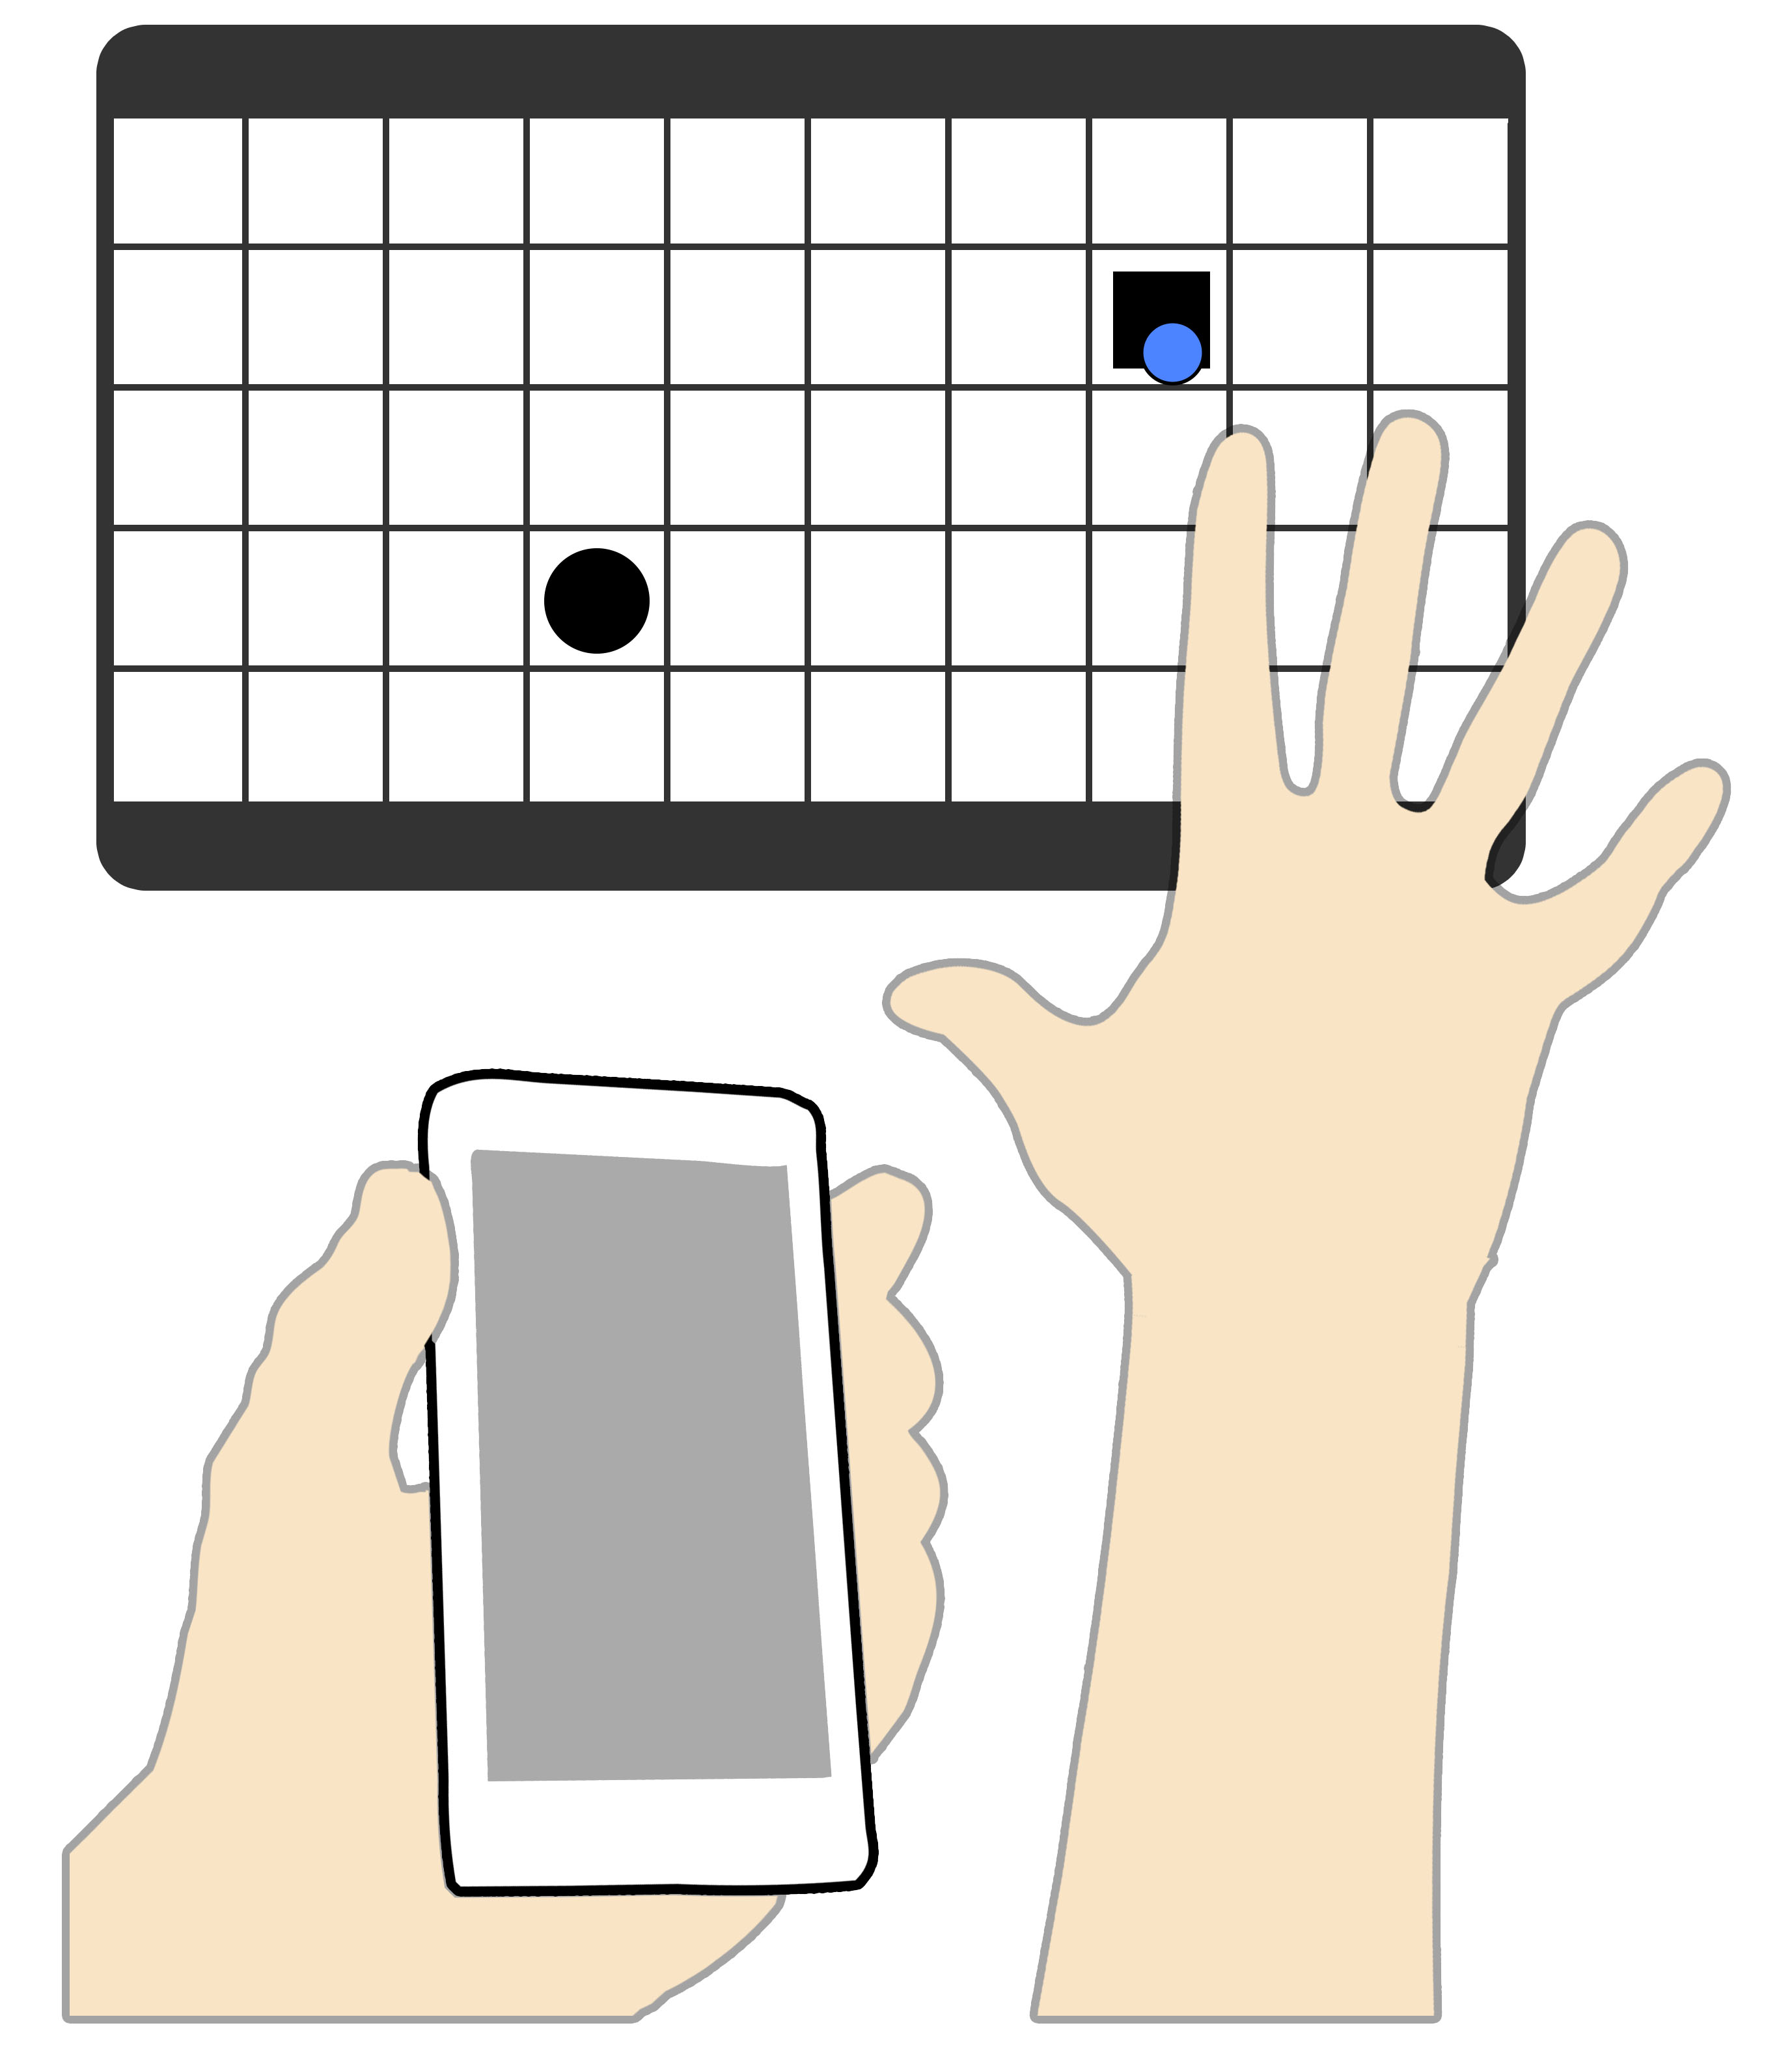
\includegraphics[width = 0.33\columnwidth]{images/techniques/grabPull1.jpg}\label{fig:grabPull1}}
	\subfloat[]{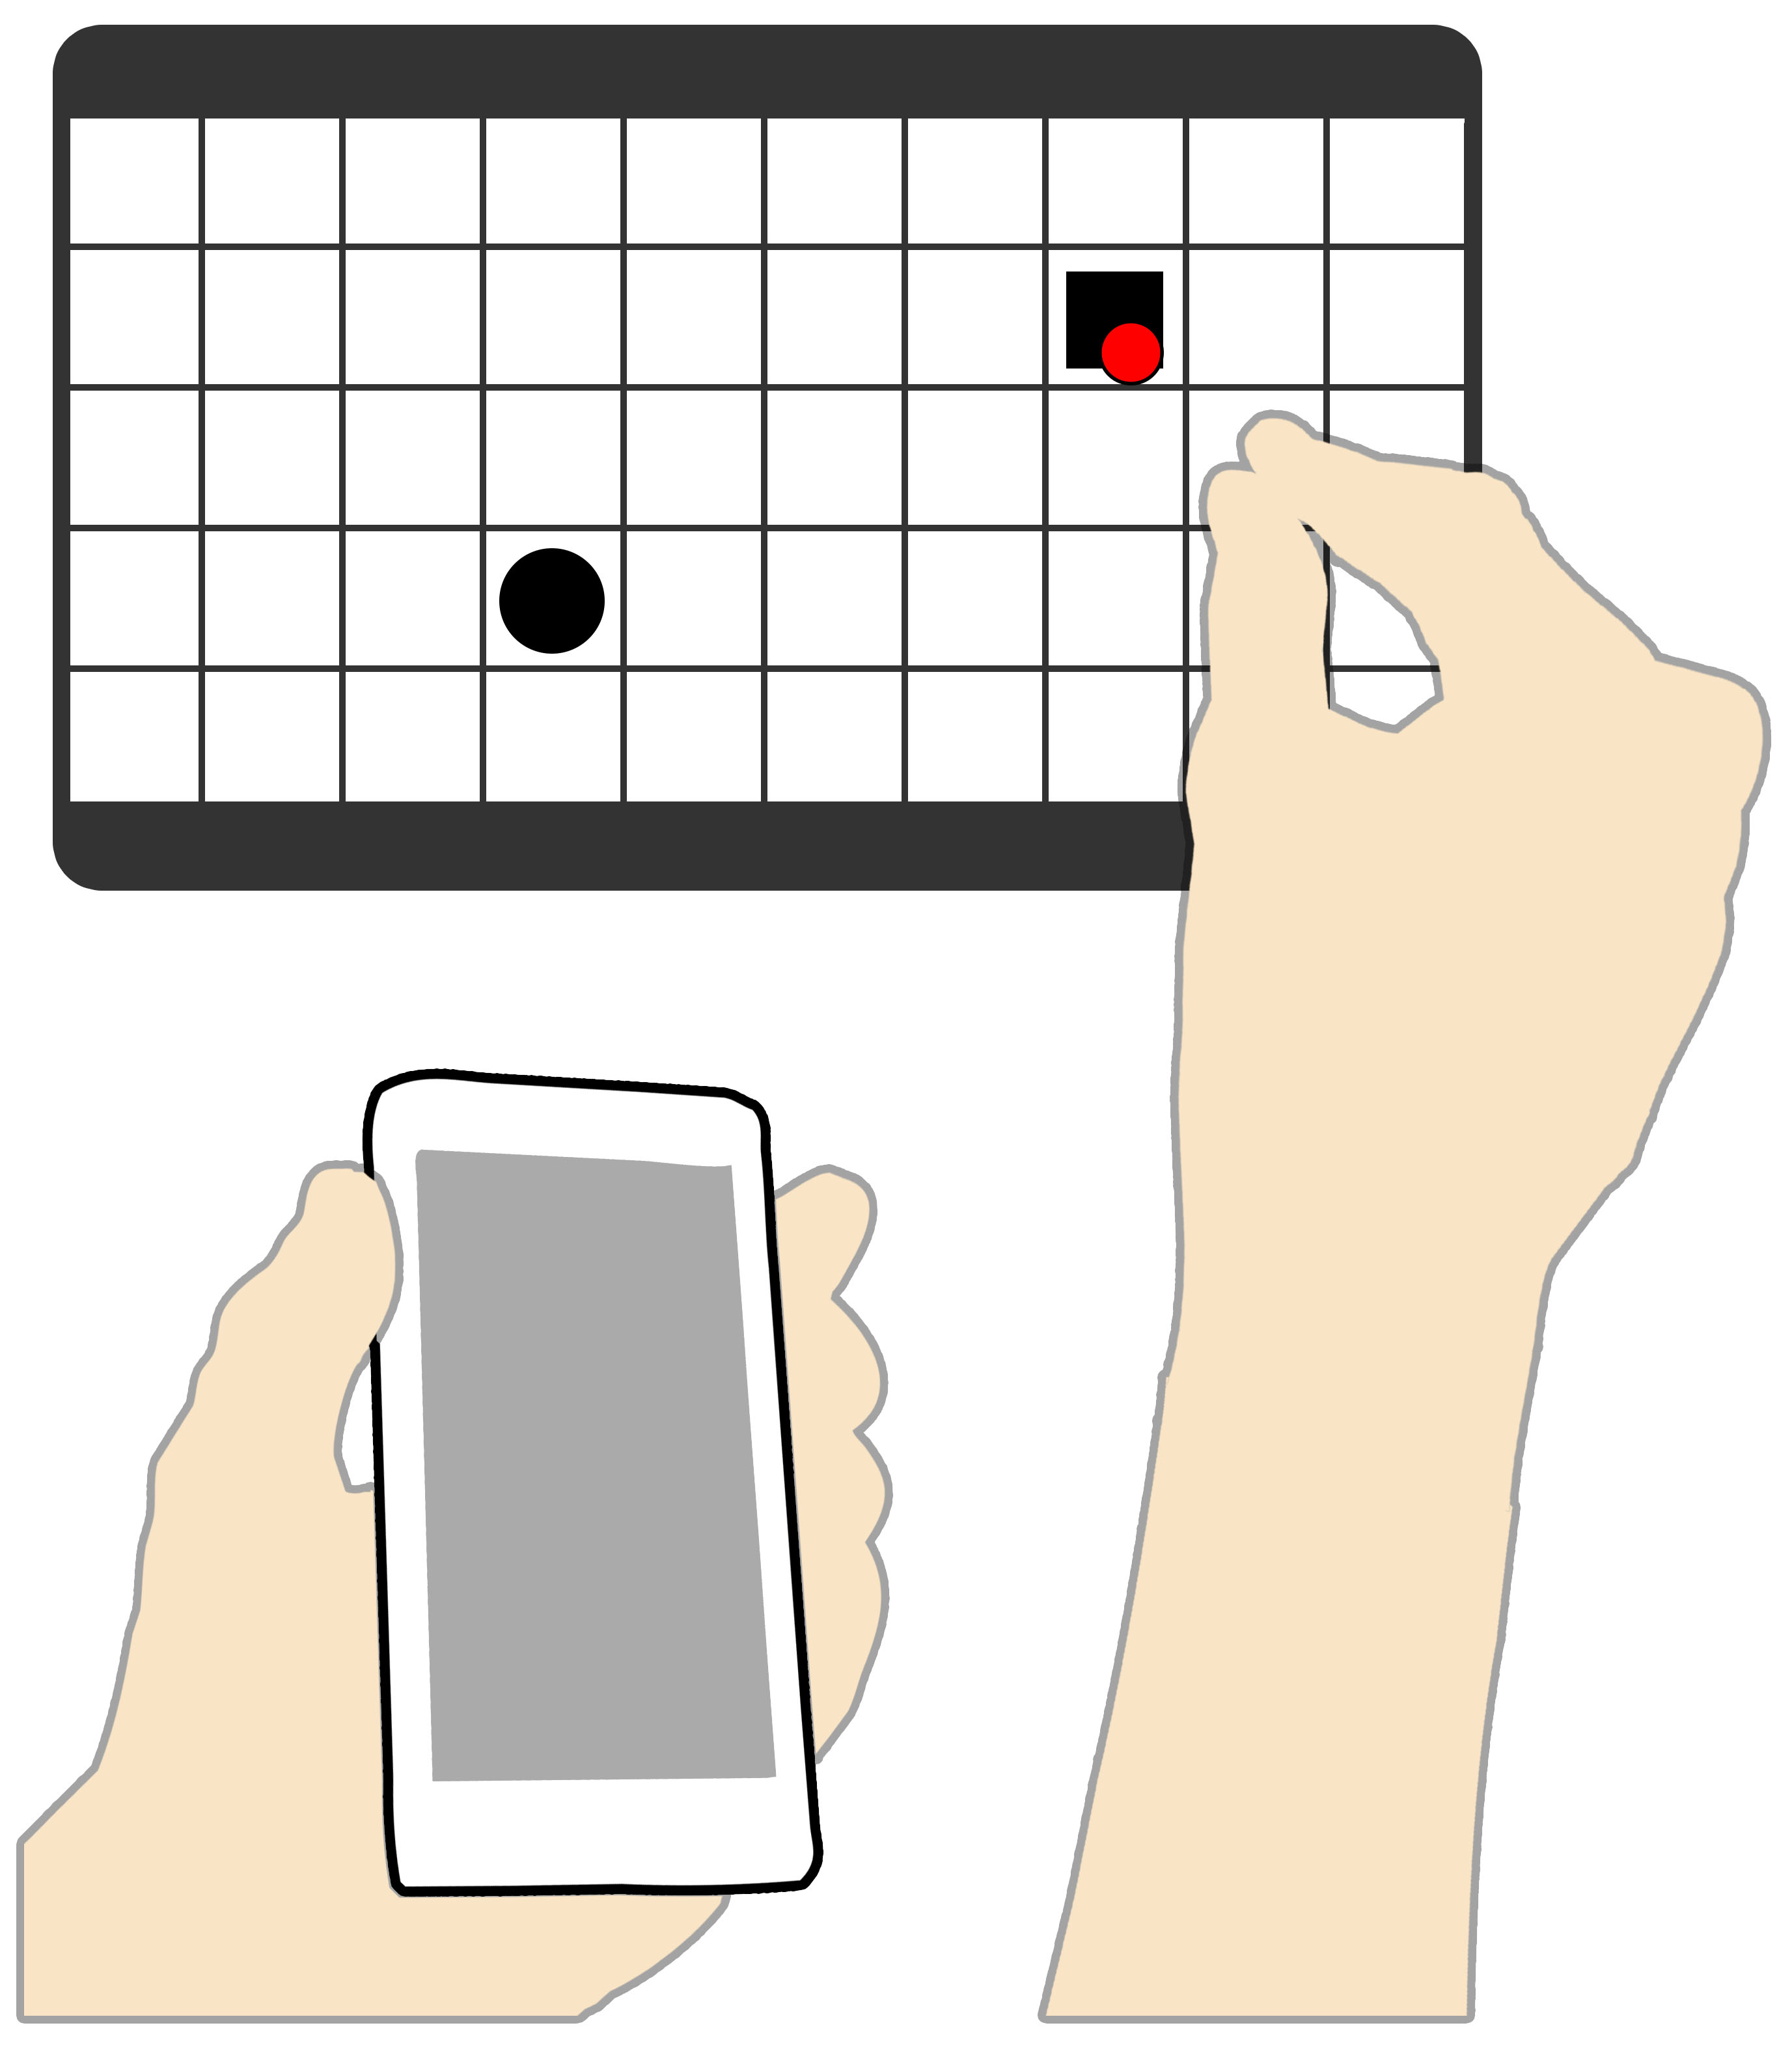
\includegraphics[width = 0.33\columnwidth]{images/techniques/grabPull2.jpg}\label{fig:grabPull2}}
	\subfloat[]{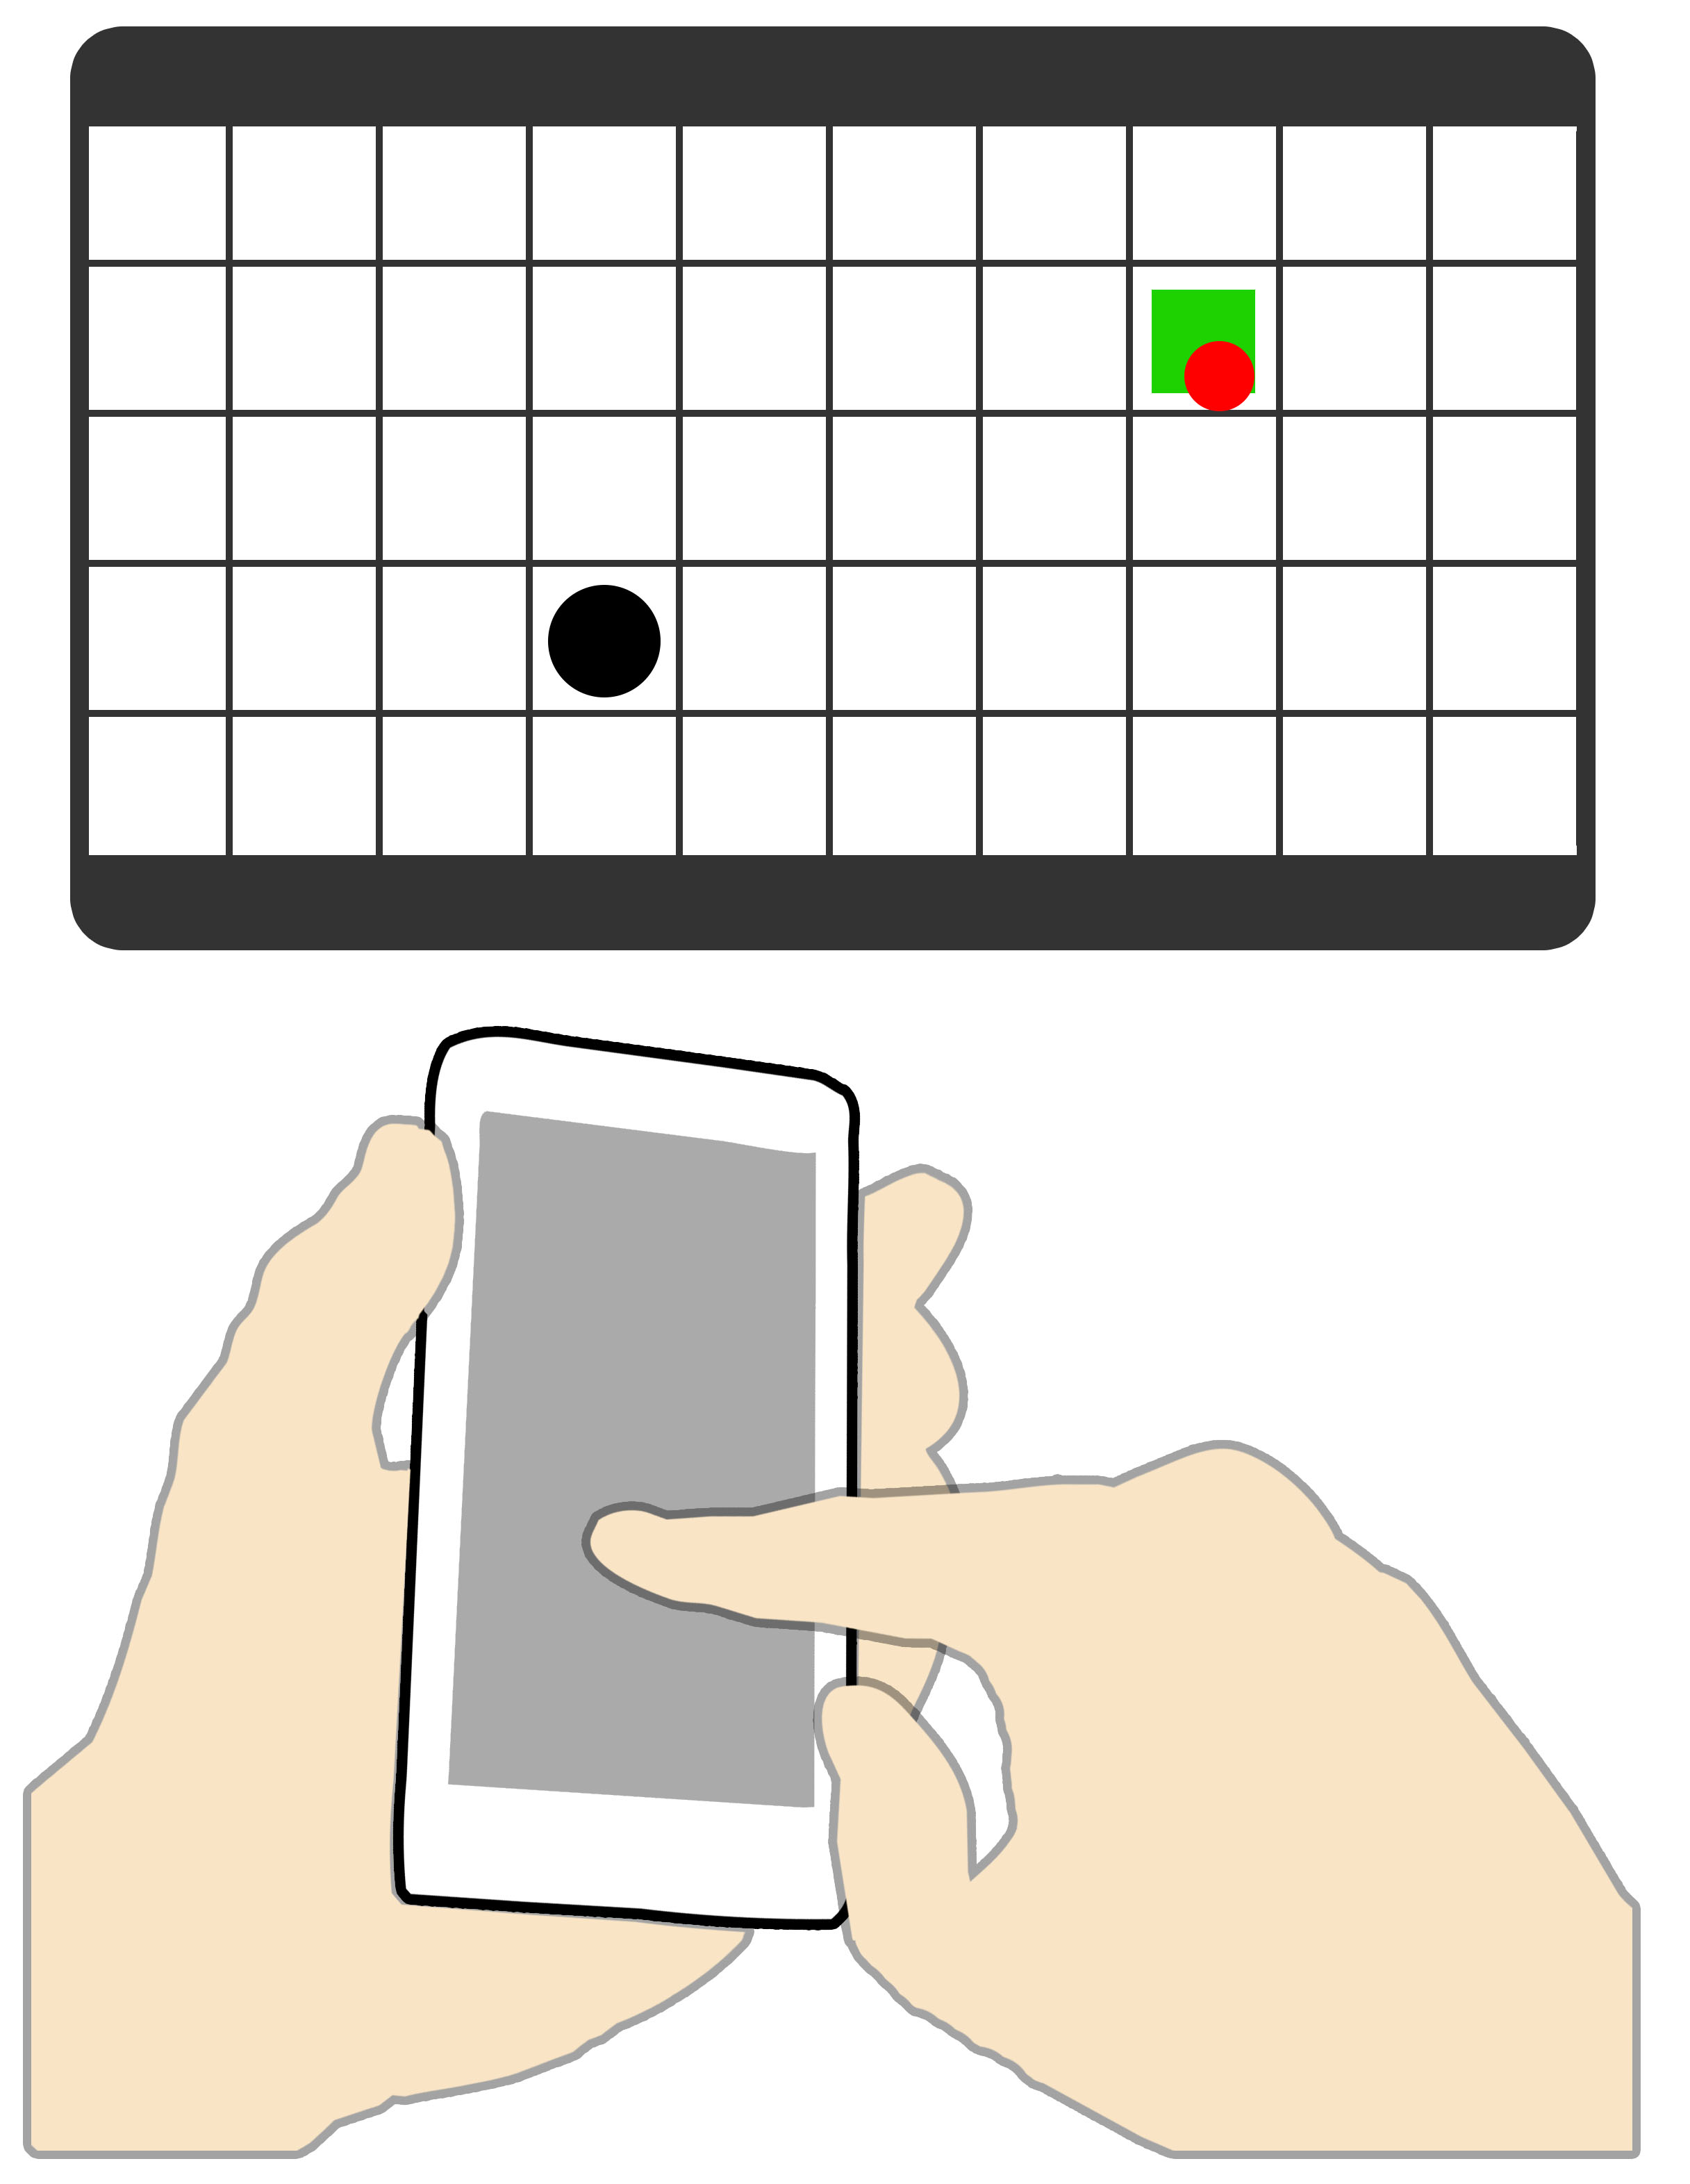
\includegraphics[width = 0.33\columnwidth]{images/techniques/grabPull3.jpg}\label{fig:grabPull3}}
	\caption{\push \grab technique}
	\label{fig:grabTechnique}
\end{figure}

\begin{figure}[H]
	\subfloat[]{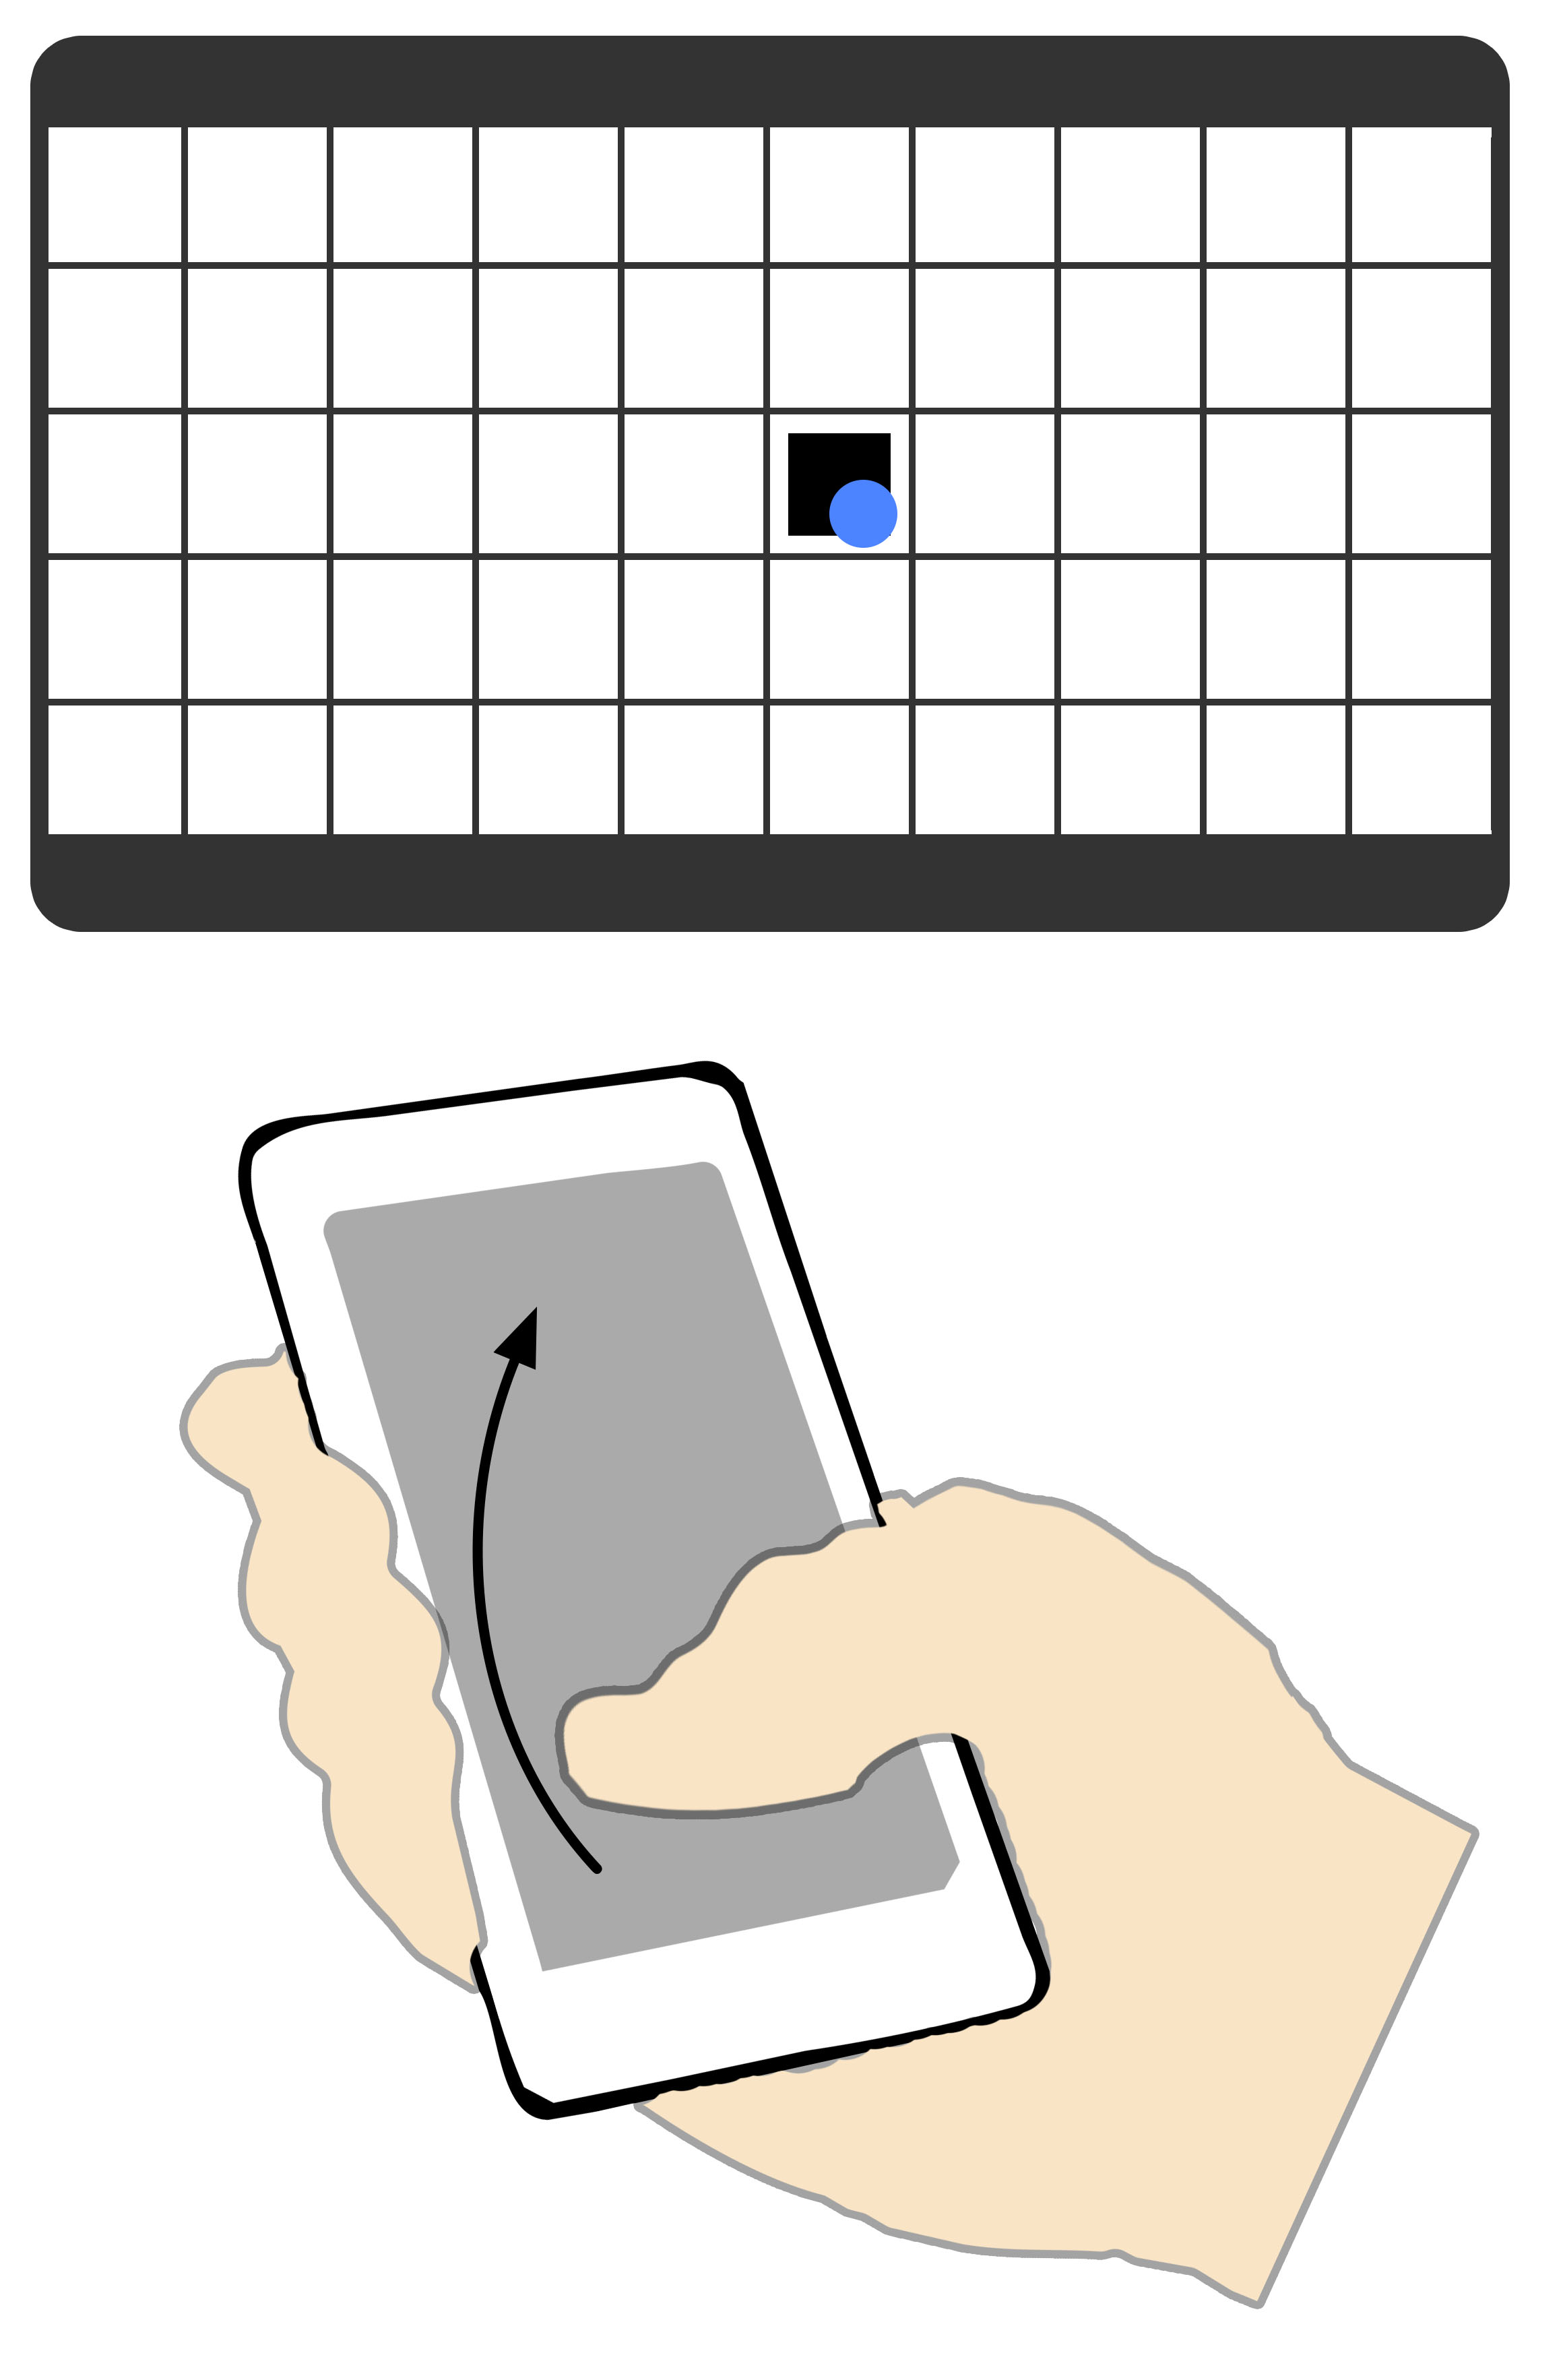
\includegraphics[width = 0.33\columnwidth]{images/techniques/swipePush1.jpg}\label{fig:swipePush1}}
	\subfloat[]{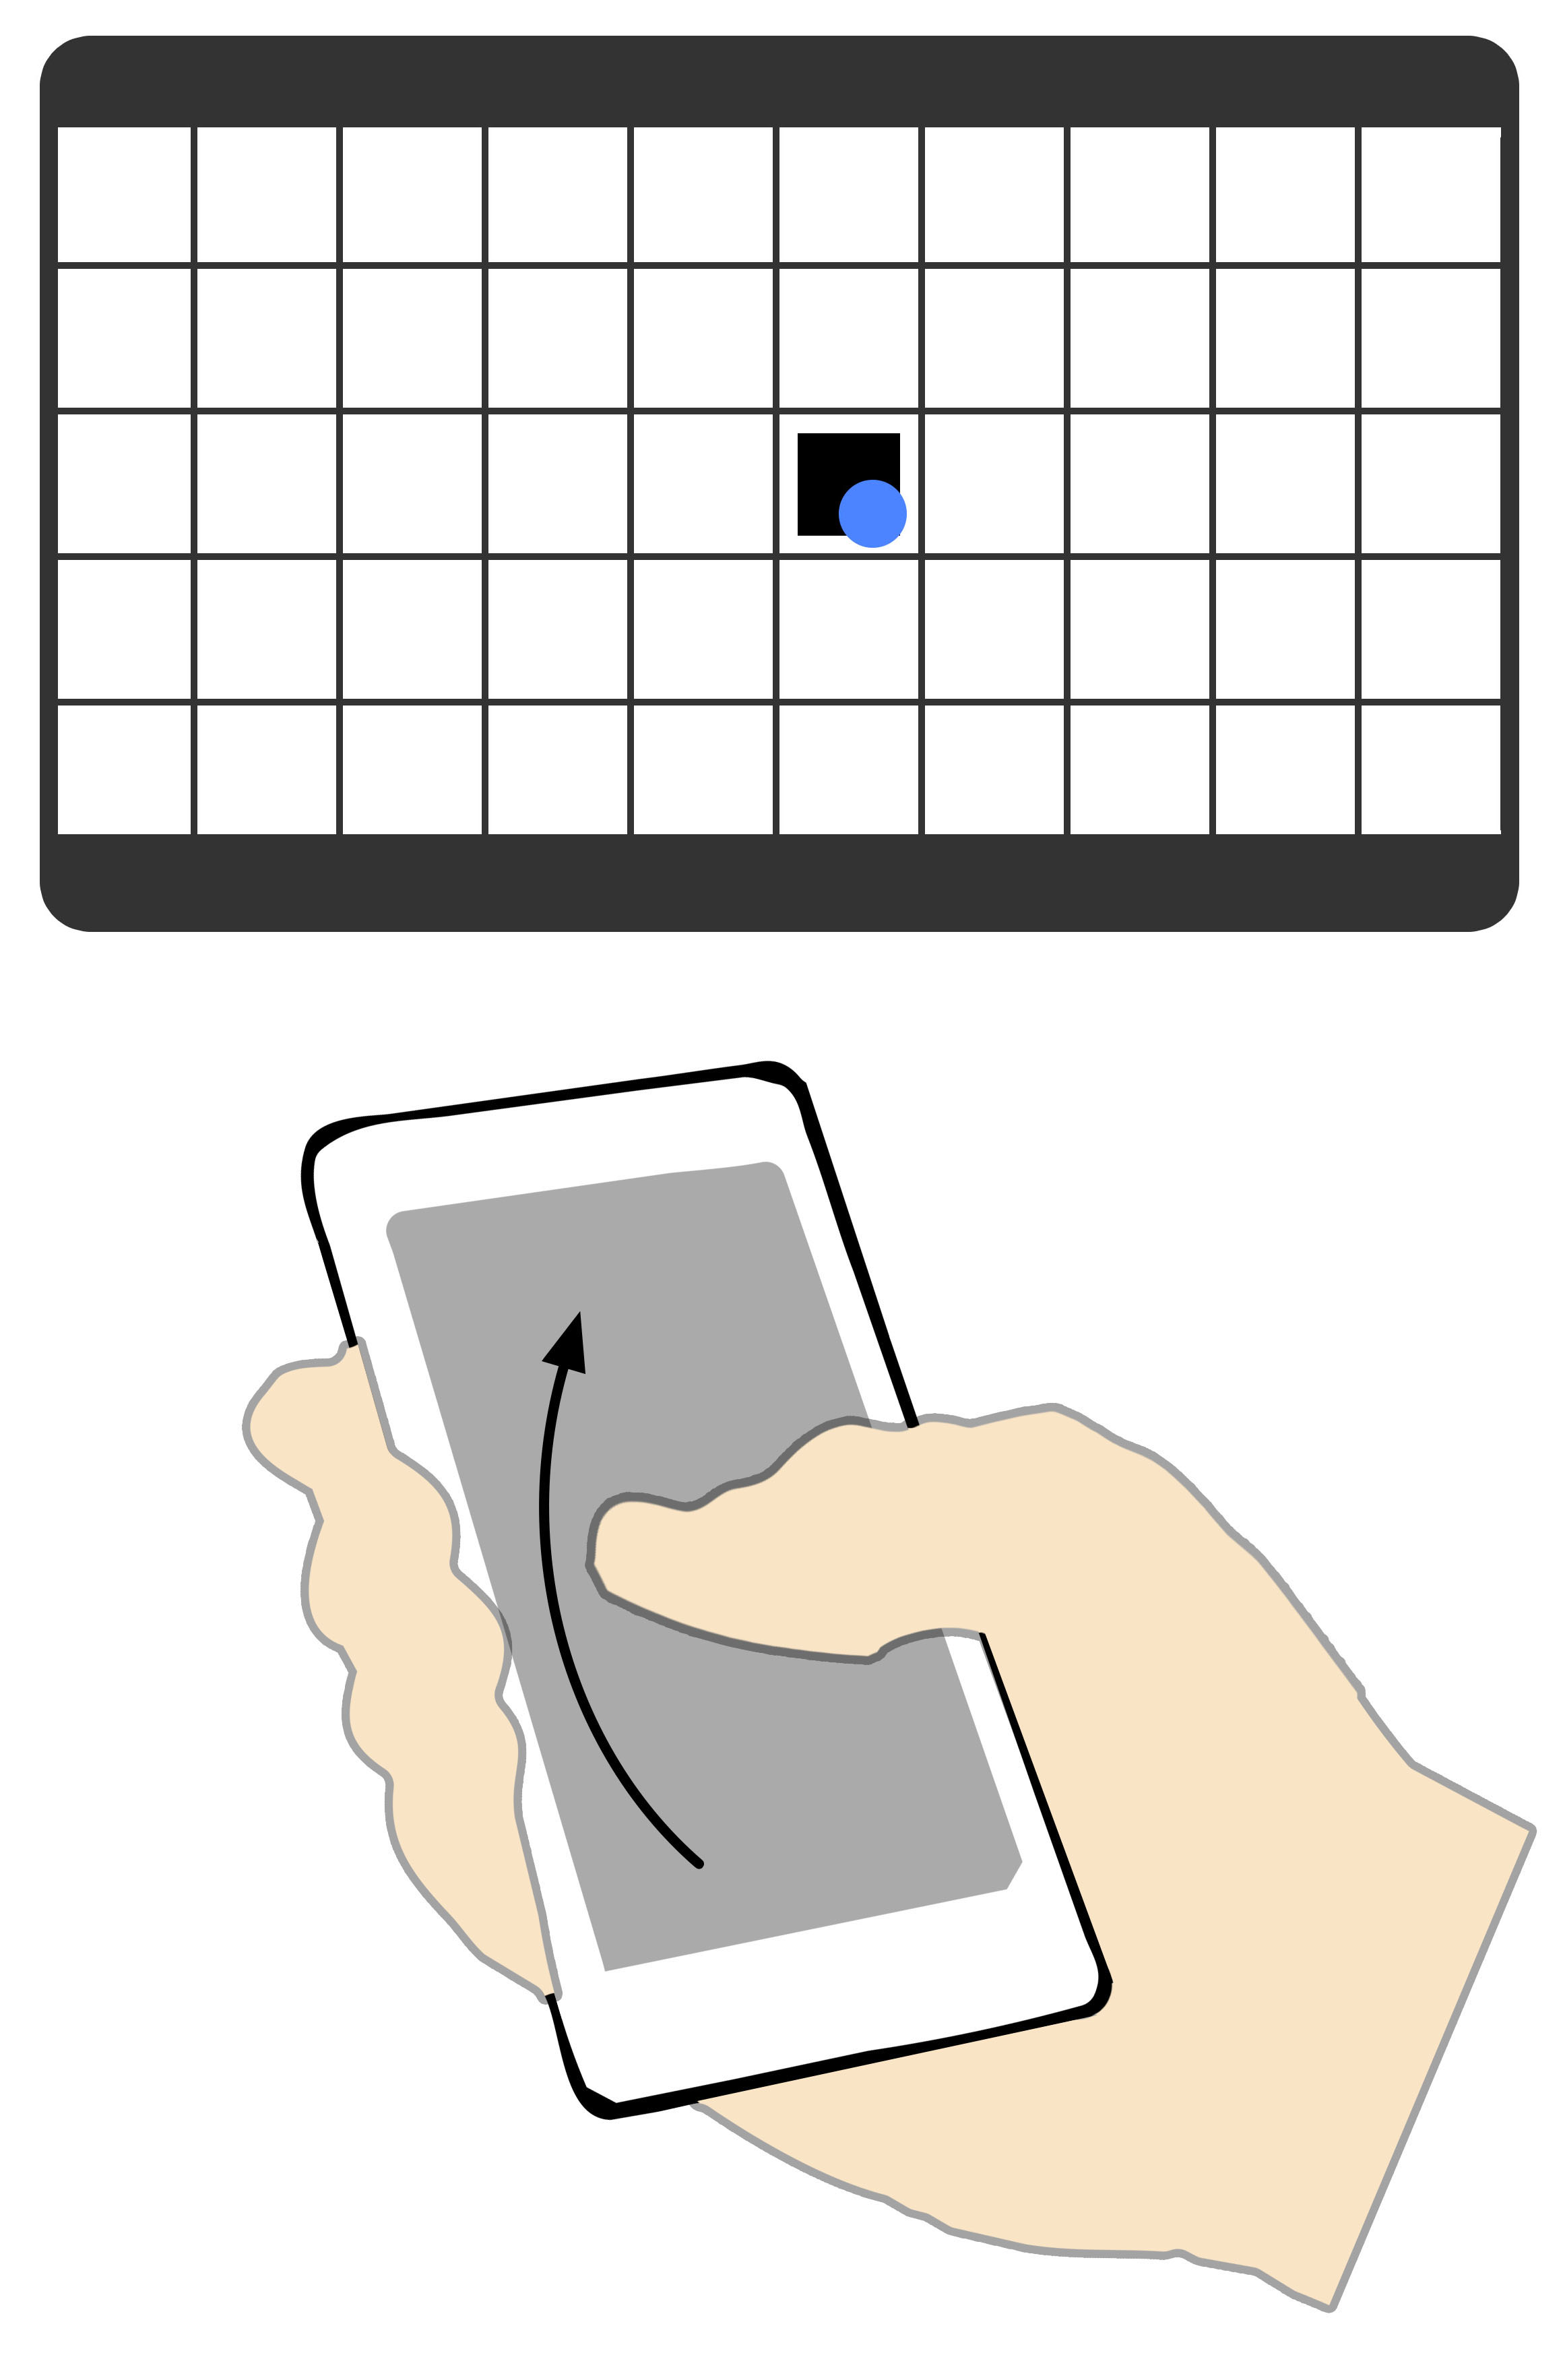
\includegraphics[width = 0.33\columnwidth]{images/techniques/swipePush2.jpg}\label{fig:swipePush2}}
	\subfloat[]{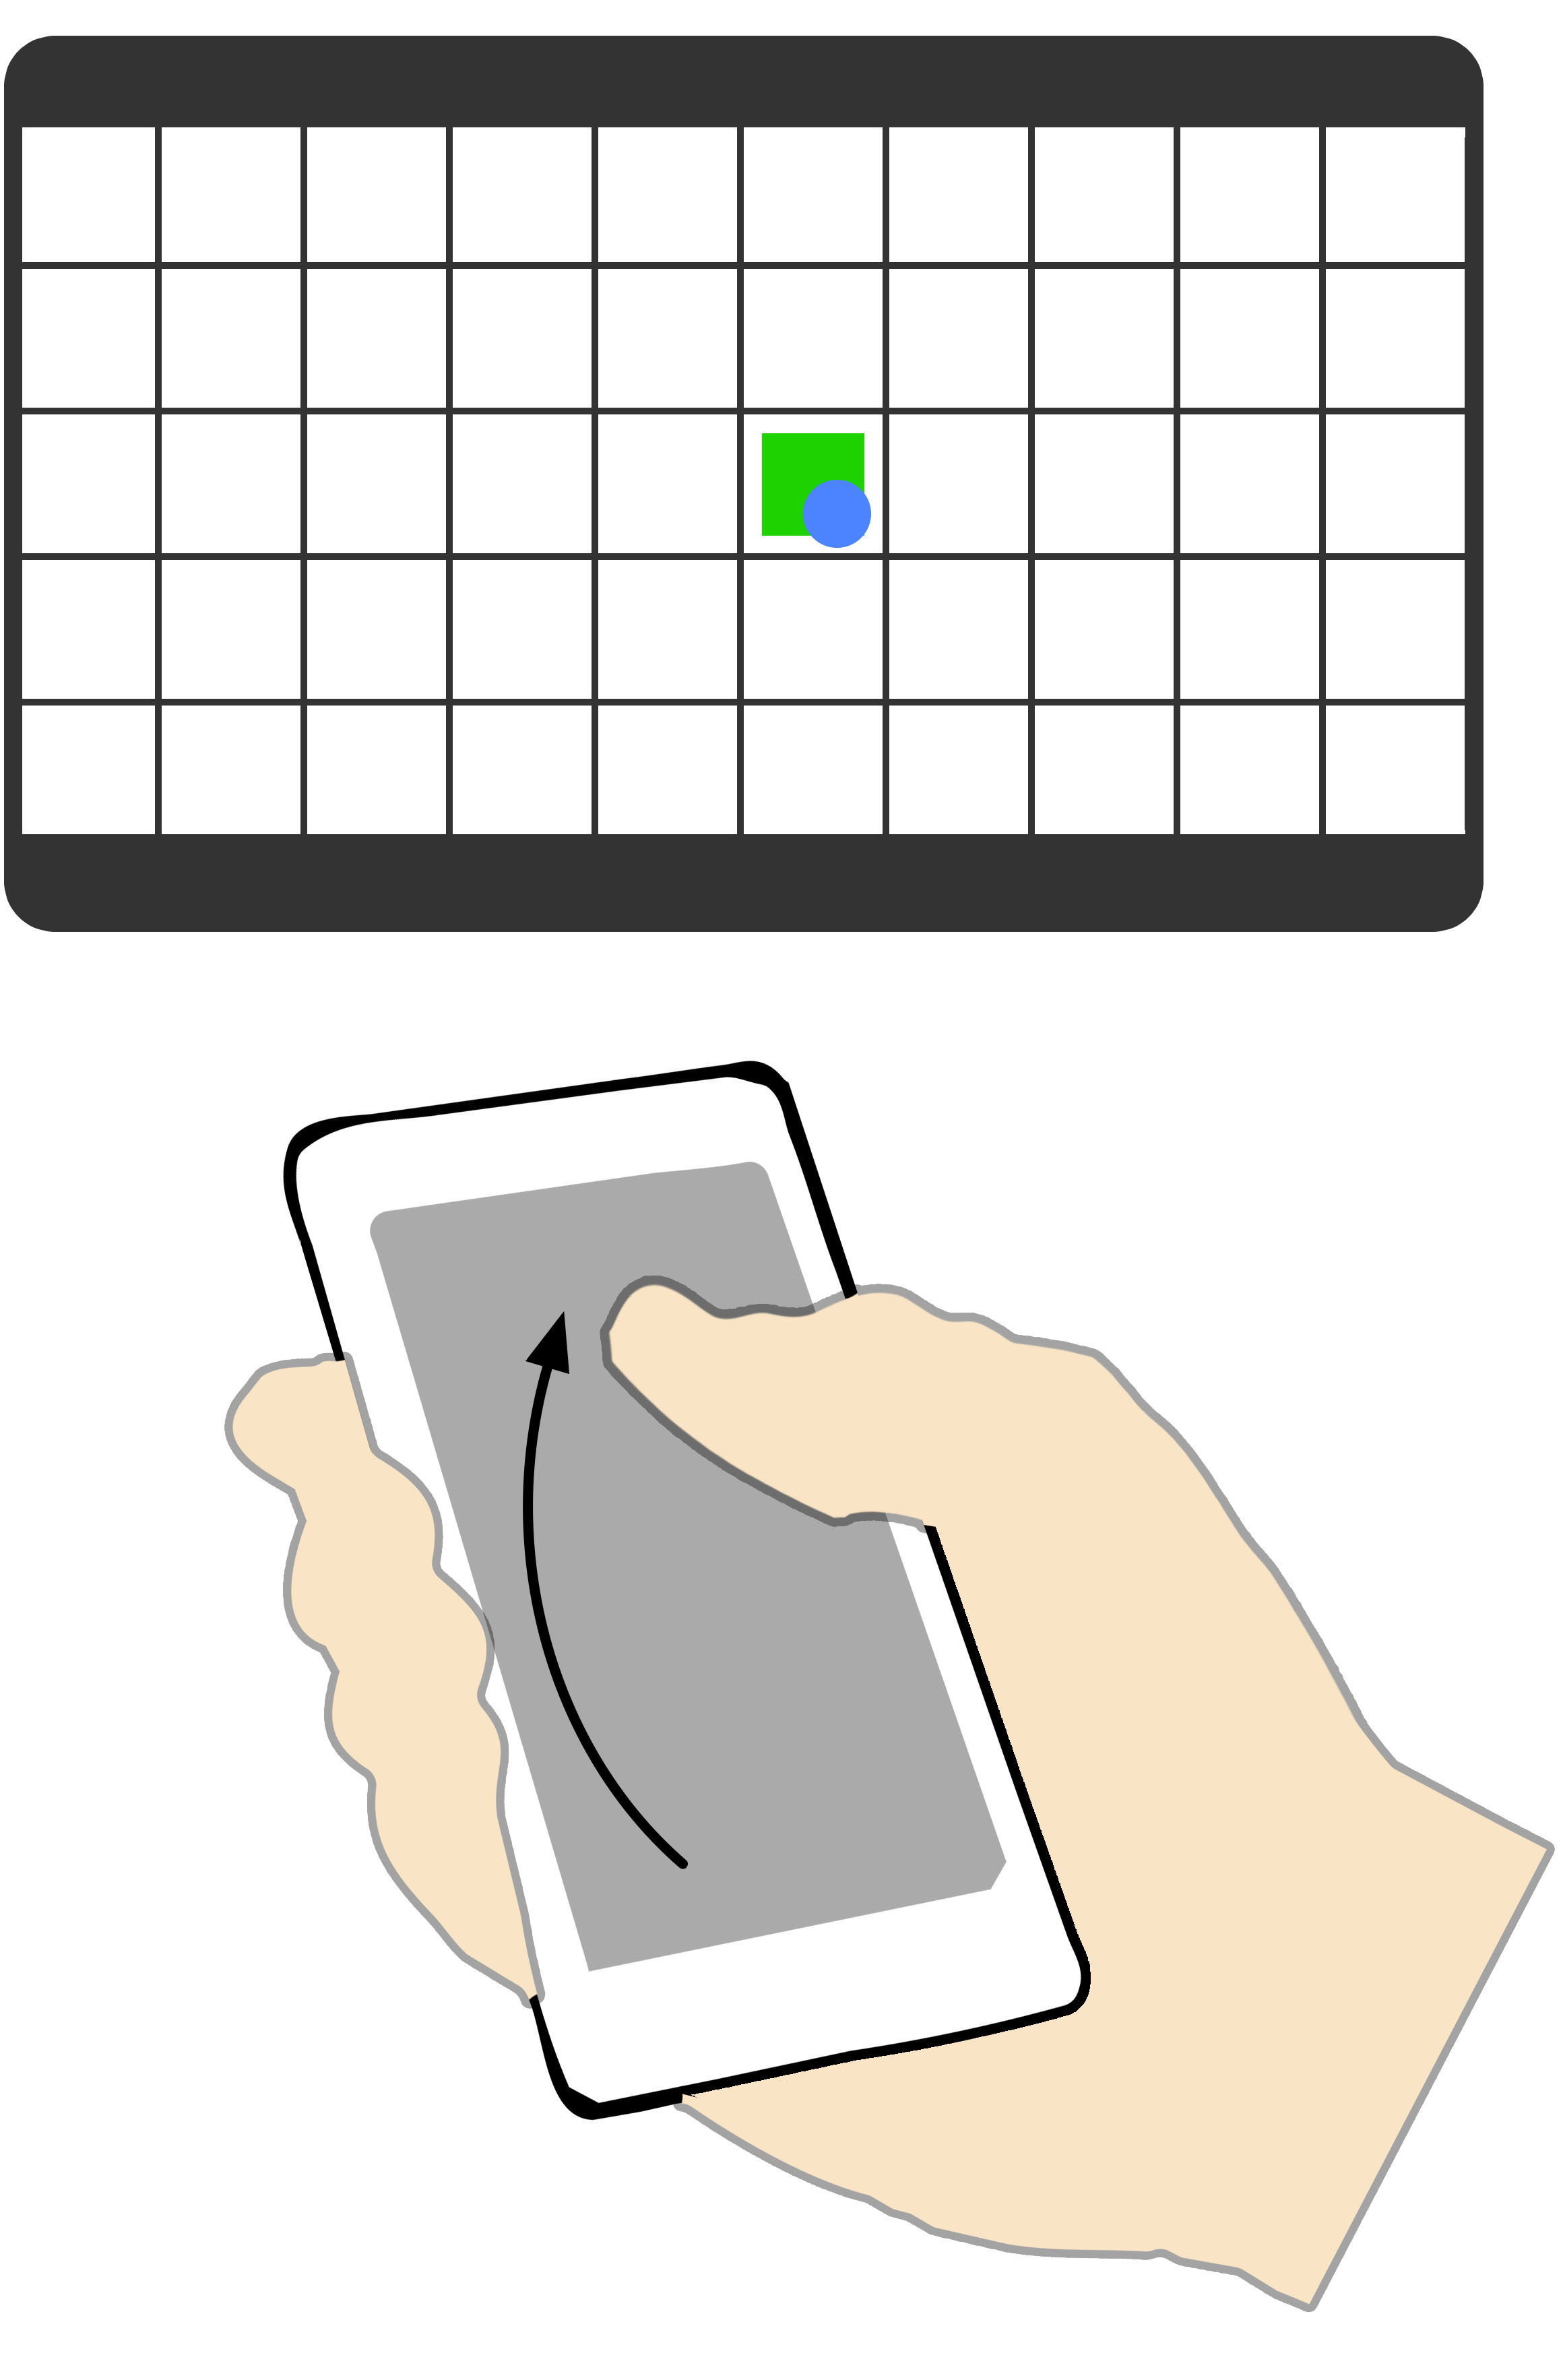
\includegraphics[width = 0.33\columnwidth]{images/techniques/swipePush3.jpg}\label{fig:swipePush3}}
	\caption{\push \grab technique}
	\label{fig:grabTechnique}
\end{figure}

\begin{figure}[H]
	\subfloat[]{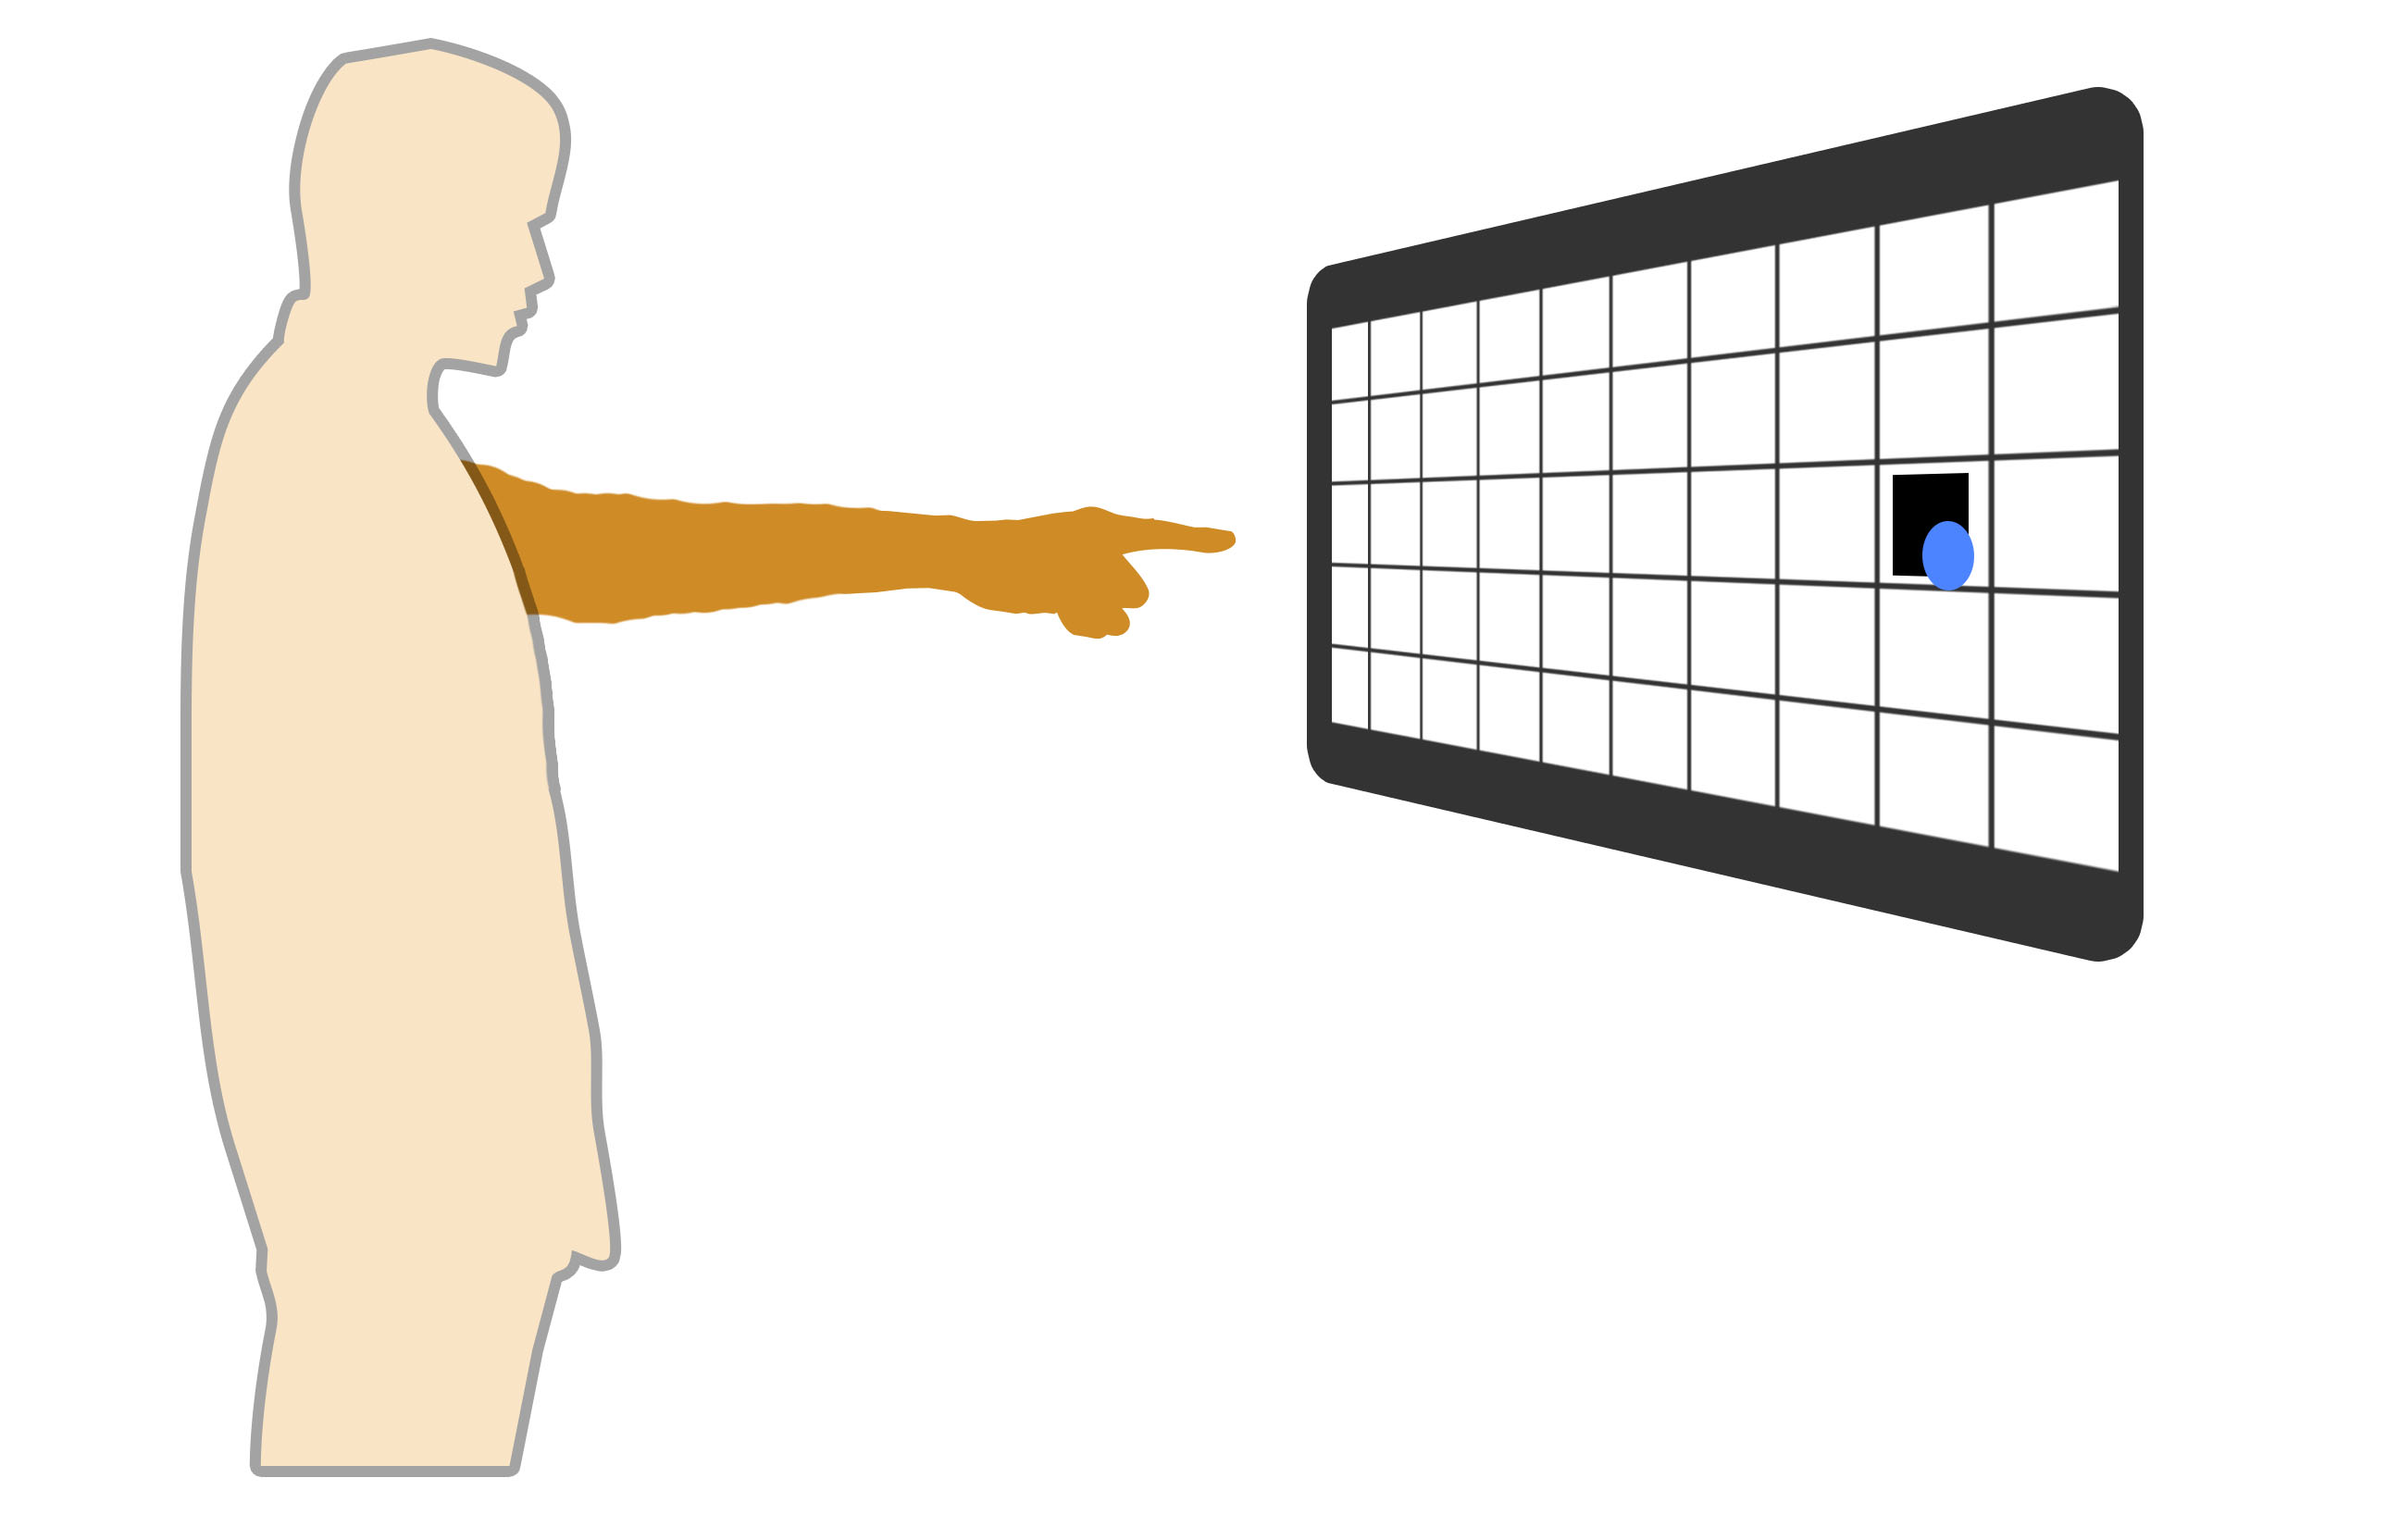
\includegraphics[width = 0.33\columnwidth]{images/techniques/throwPush1.jpg}\label{fig:throwPush1}}
	\subfloat[]{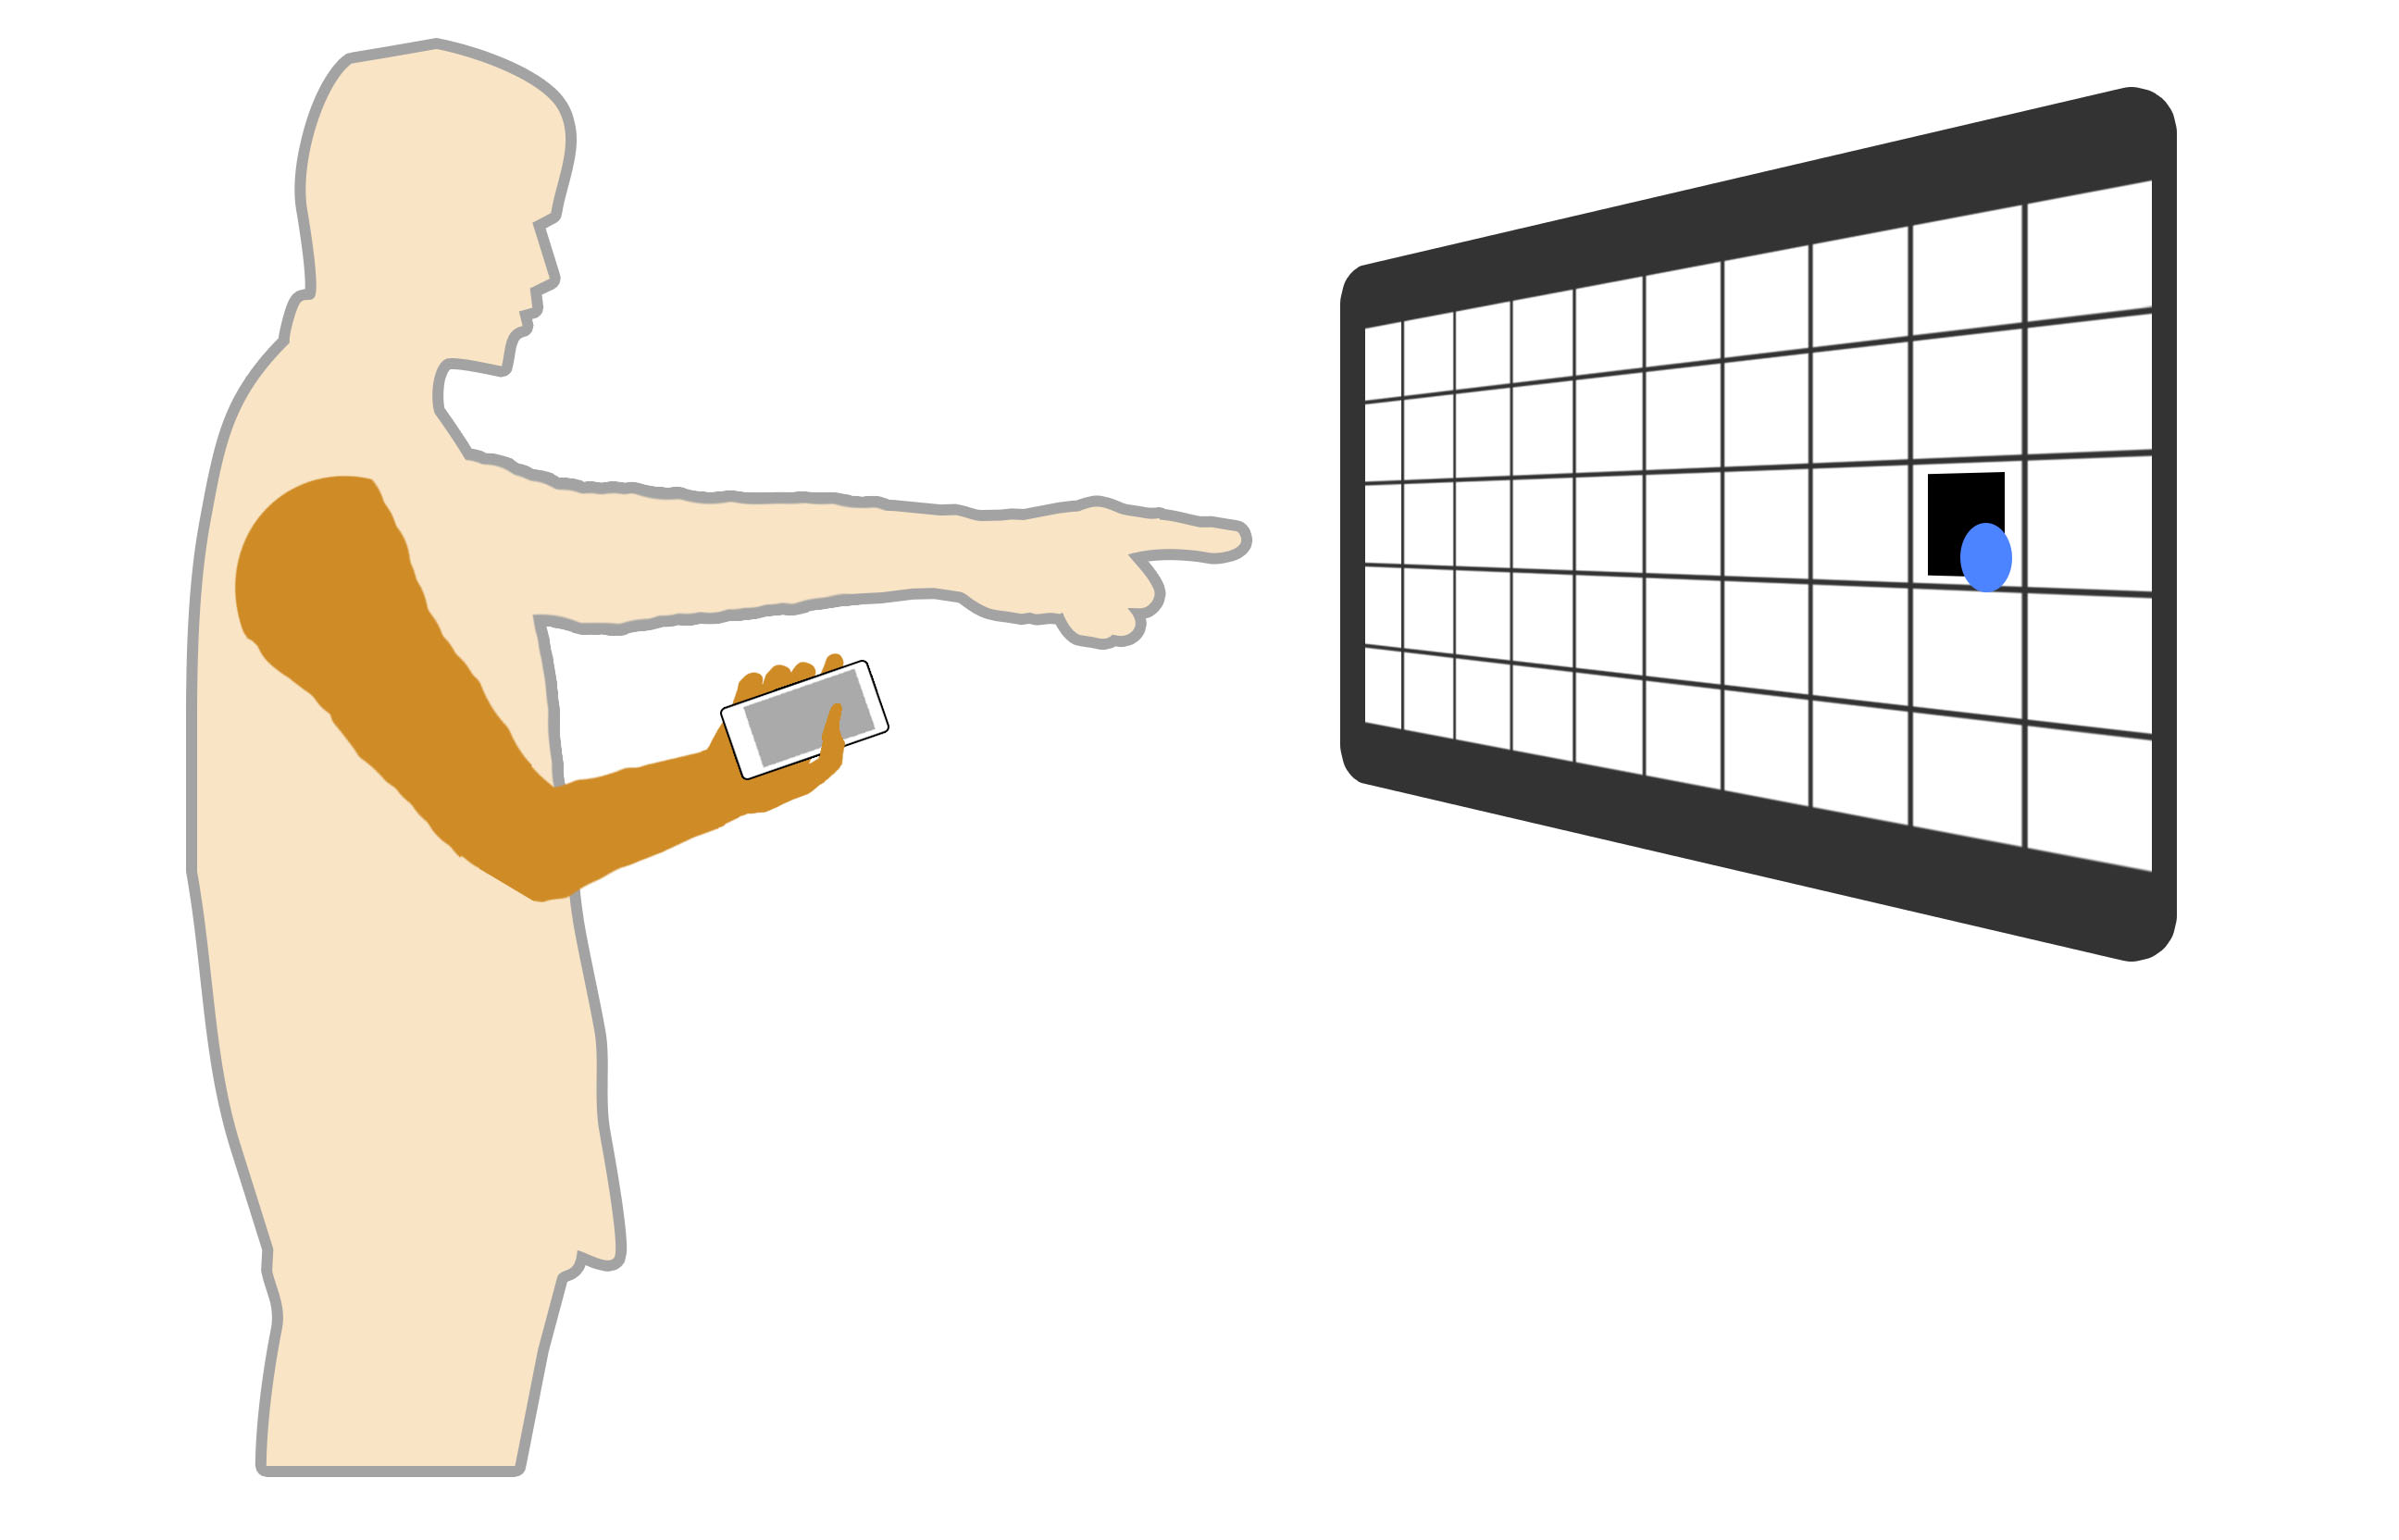
\includegraphics[width = 0.33\columnwidth]{images/techniques/throwPush2.jpg}\label{fig:throwPush2}}
	\subfloat[]{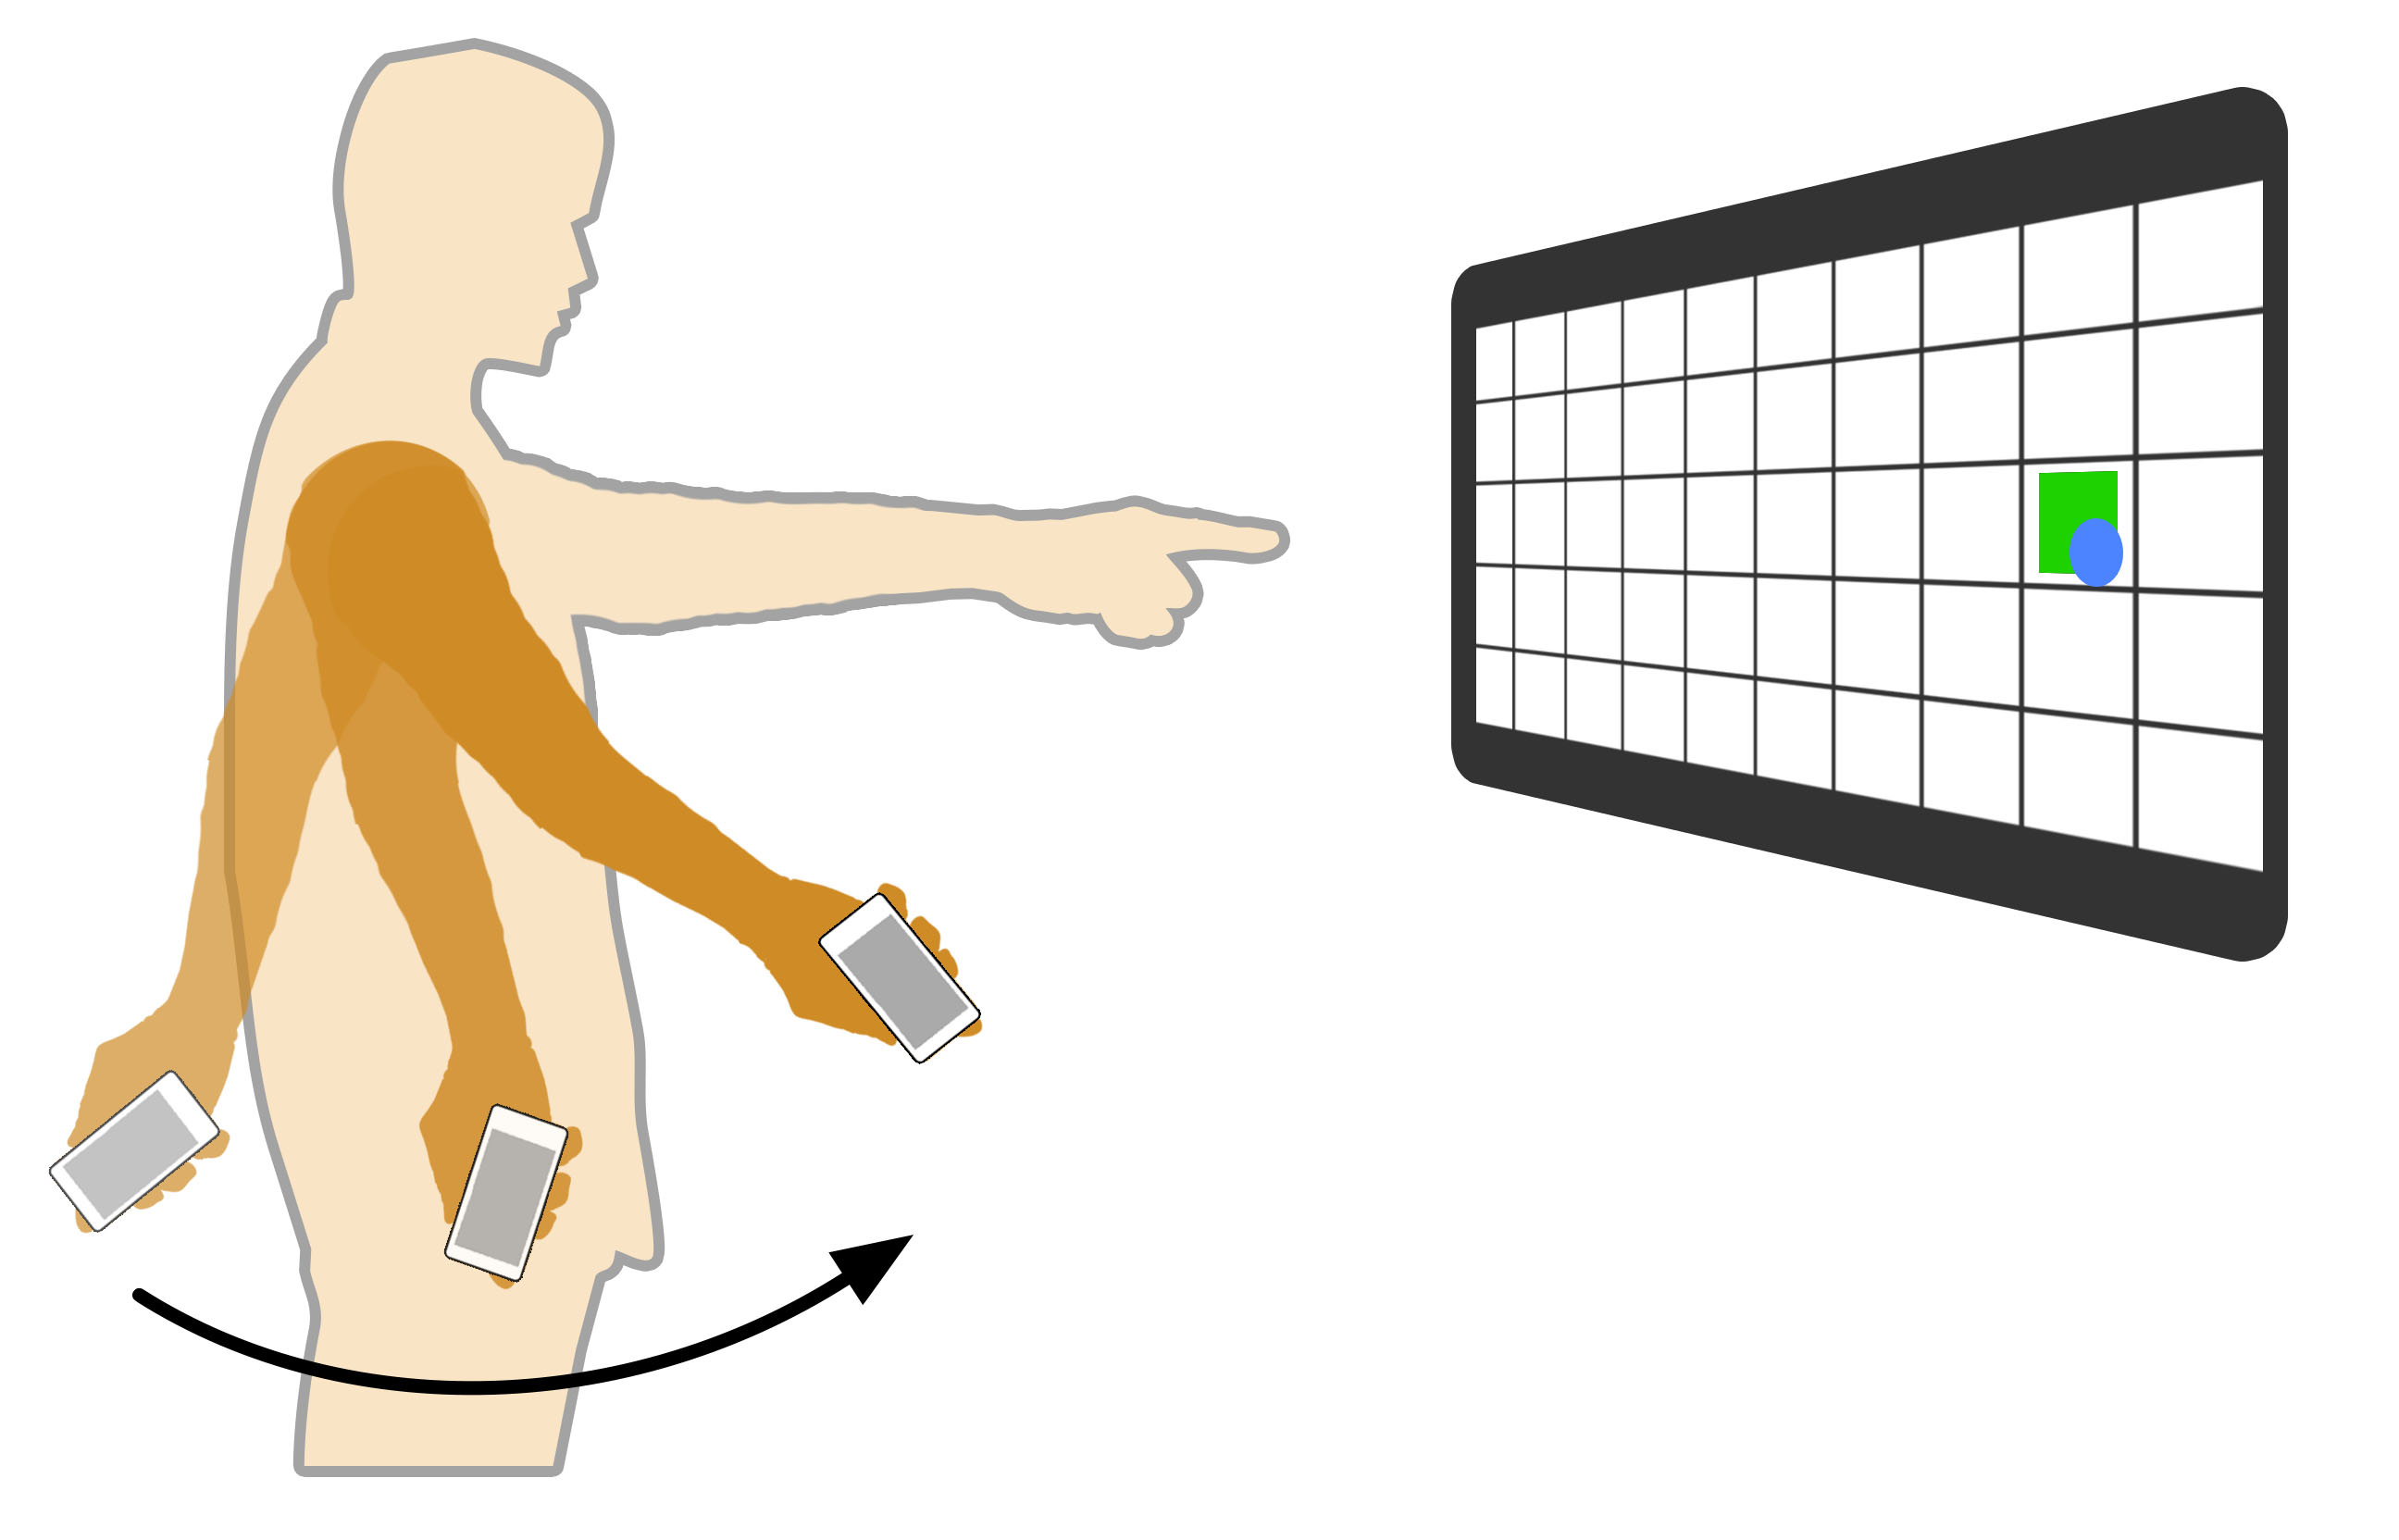
\includegraphics[width = 0.33\columnwidth]{images/techniques/throwPush3.jpg}\label{fig:throwPush3}}
	\caption{\push \grab technique}
	\label{fig:grabTechnique}
\end{figure}

\begin{figure}[H]
	\subfloat[]{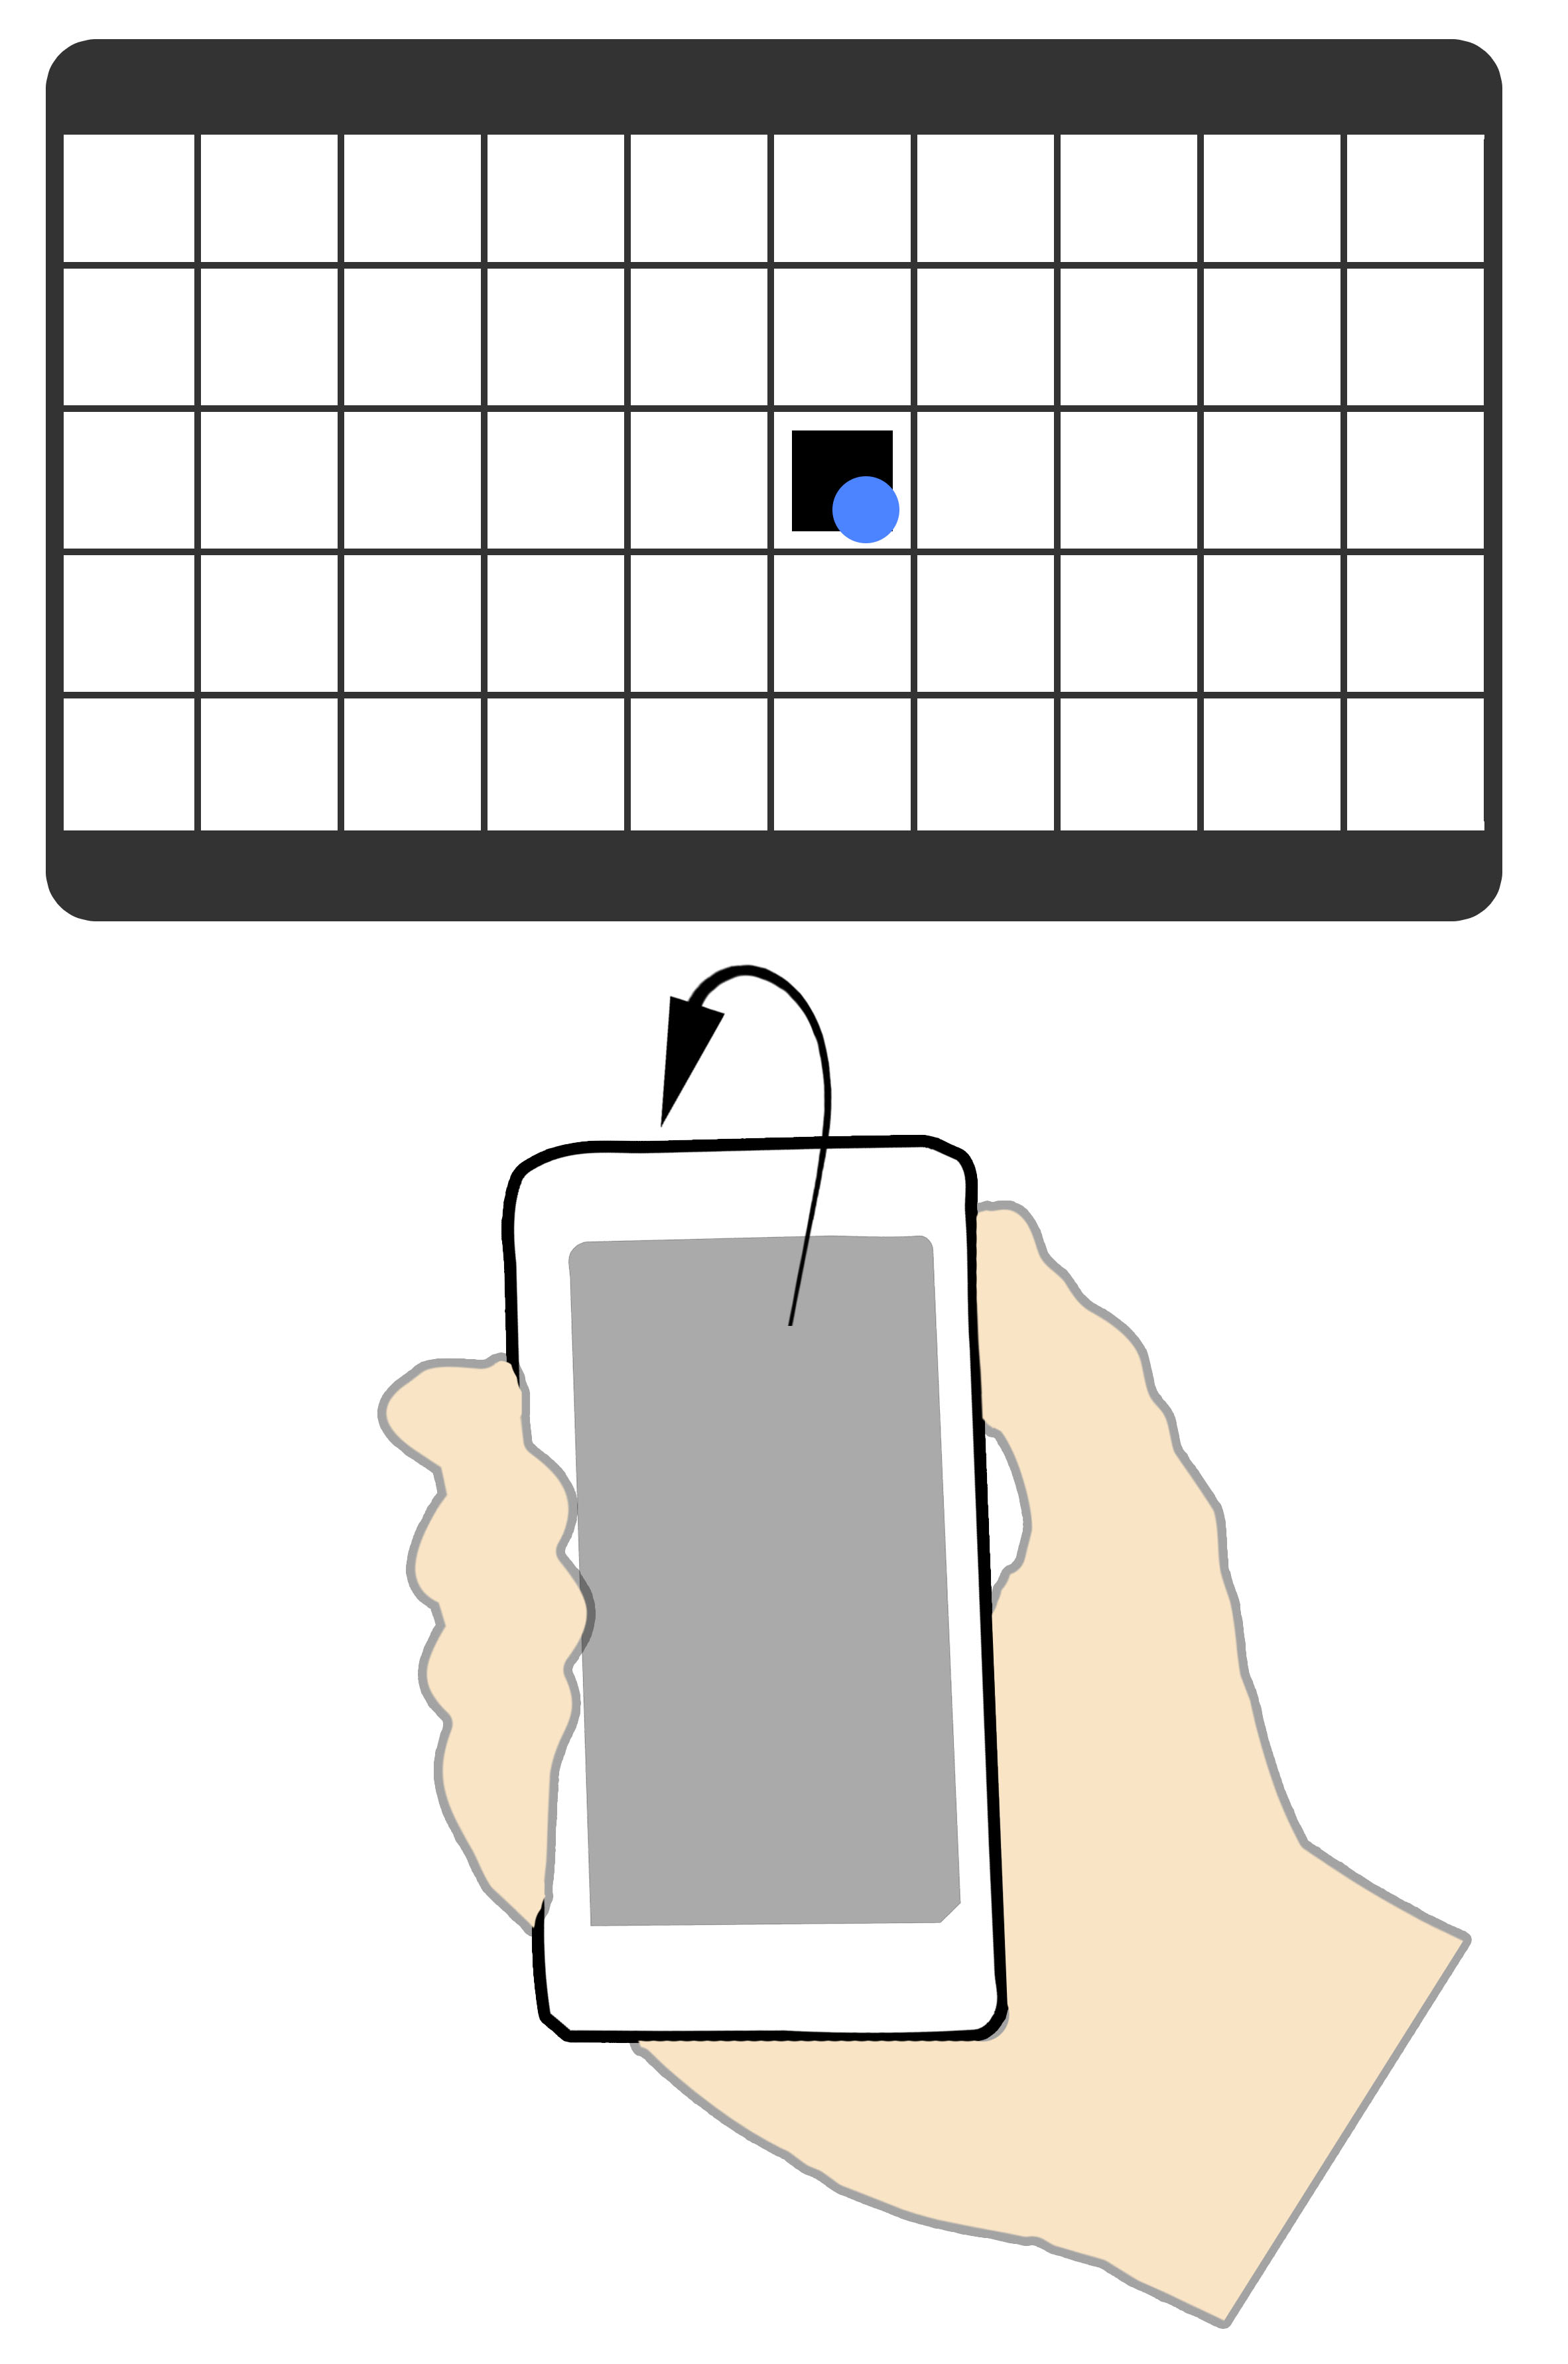
\includegraphics[width = 0.33\columnwidth]{images/techniques/tiltPush1.jpg}\label{fig:tiltPush1}}
	\subfloat[]{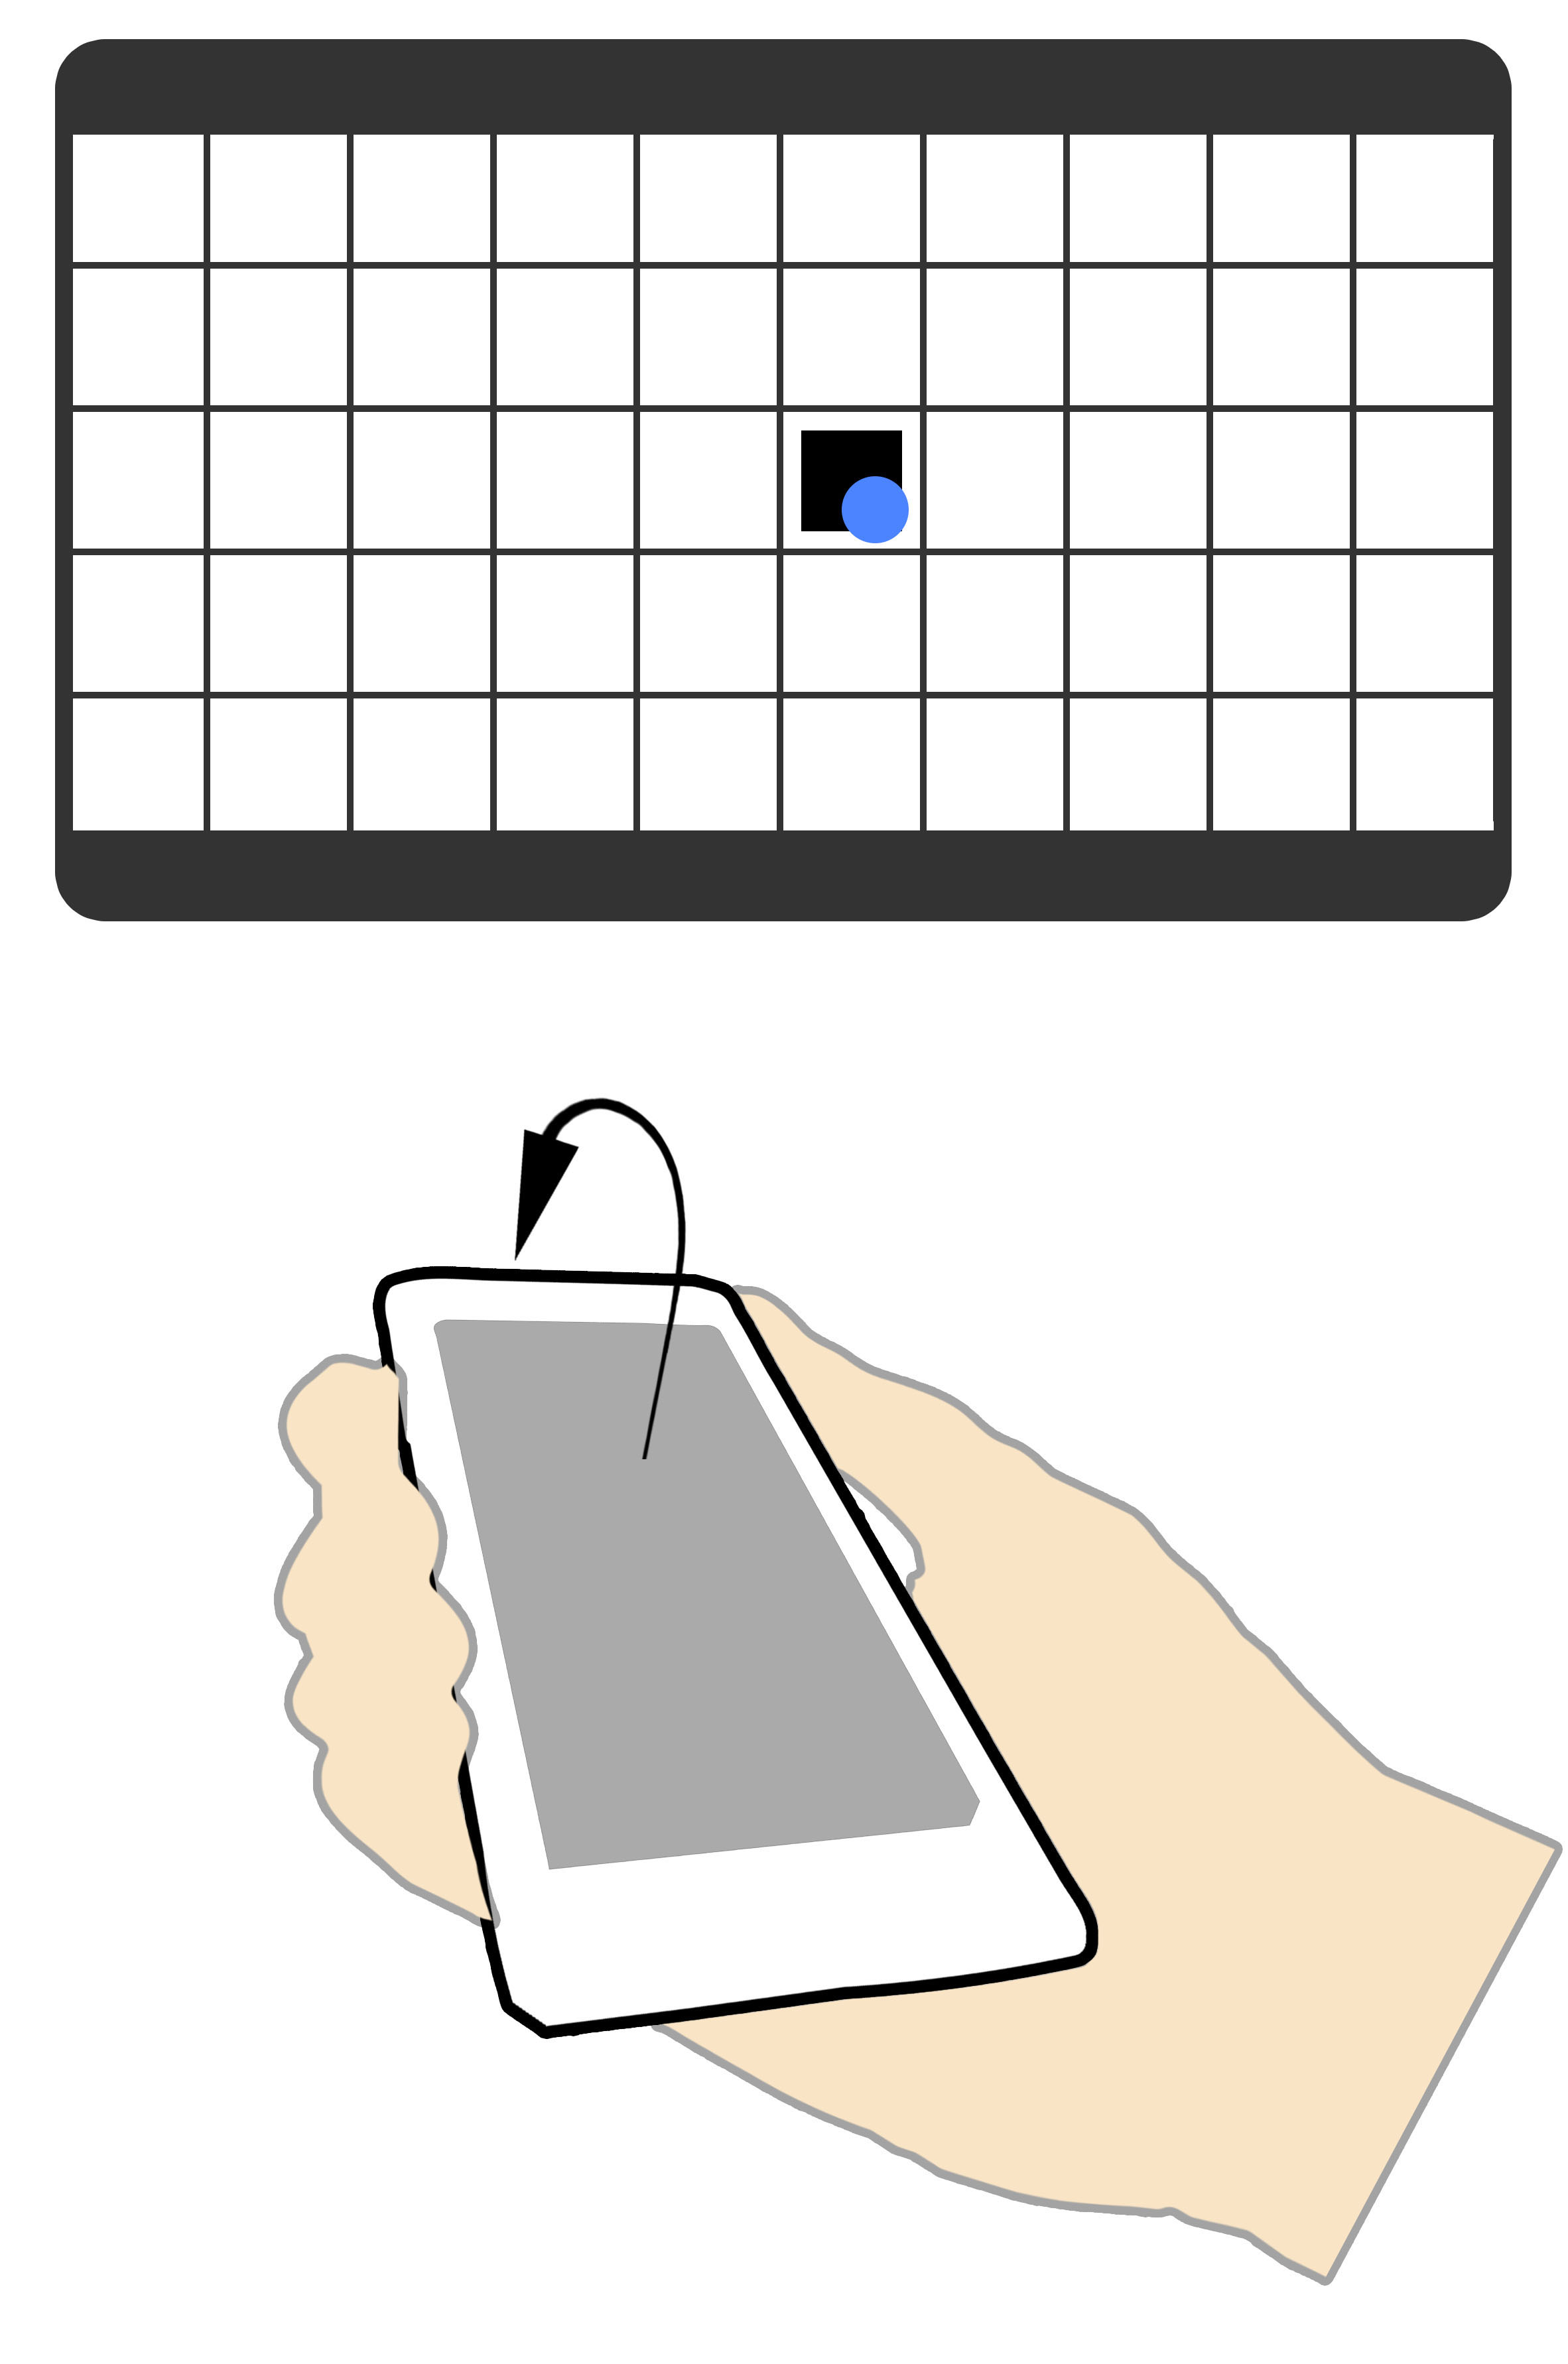
\includegraphics[width = 0.33\columnwidth]{images/techniques/tiltPush2.jpg}\label{fig:tiltPush2}}
	\subfloat[]{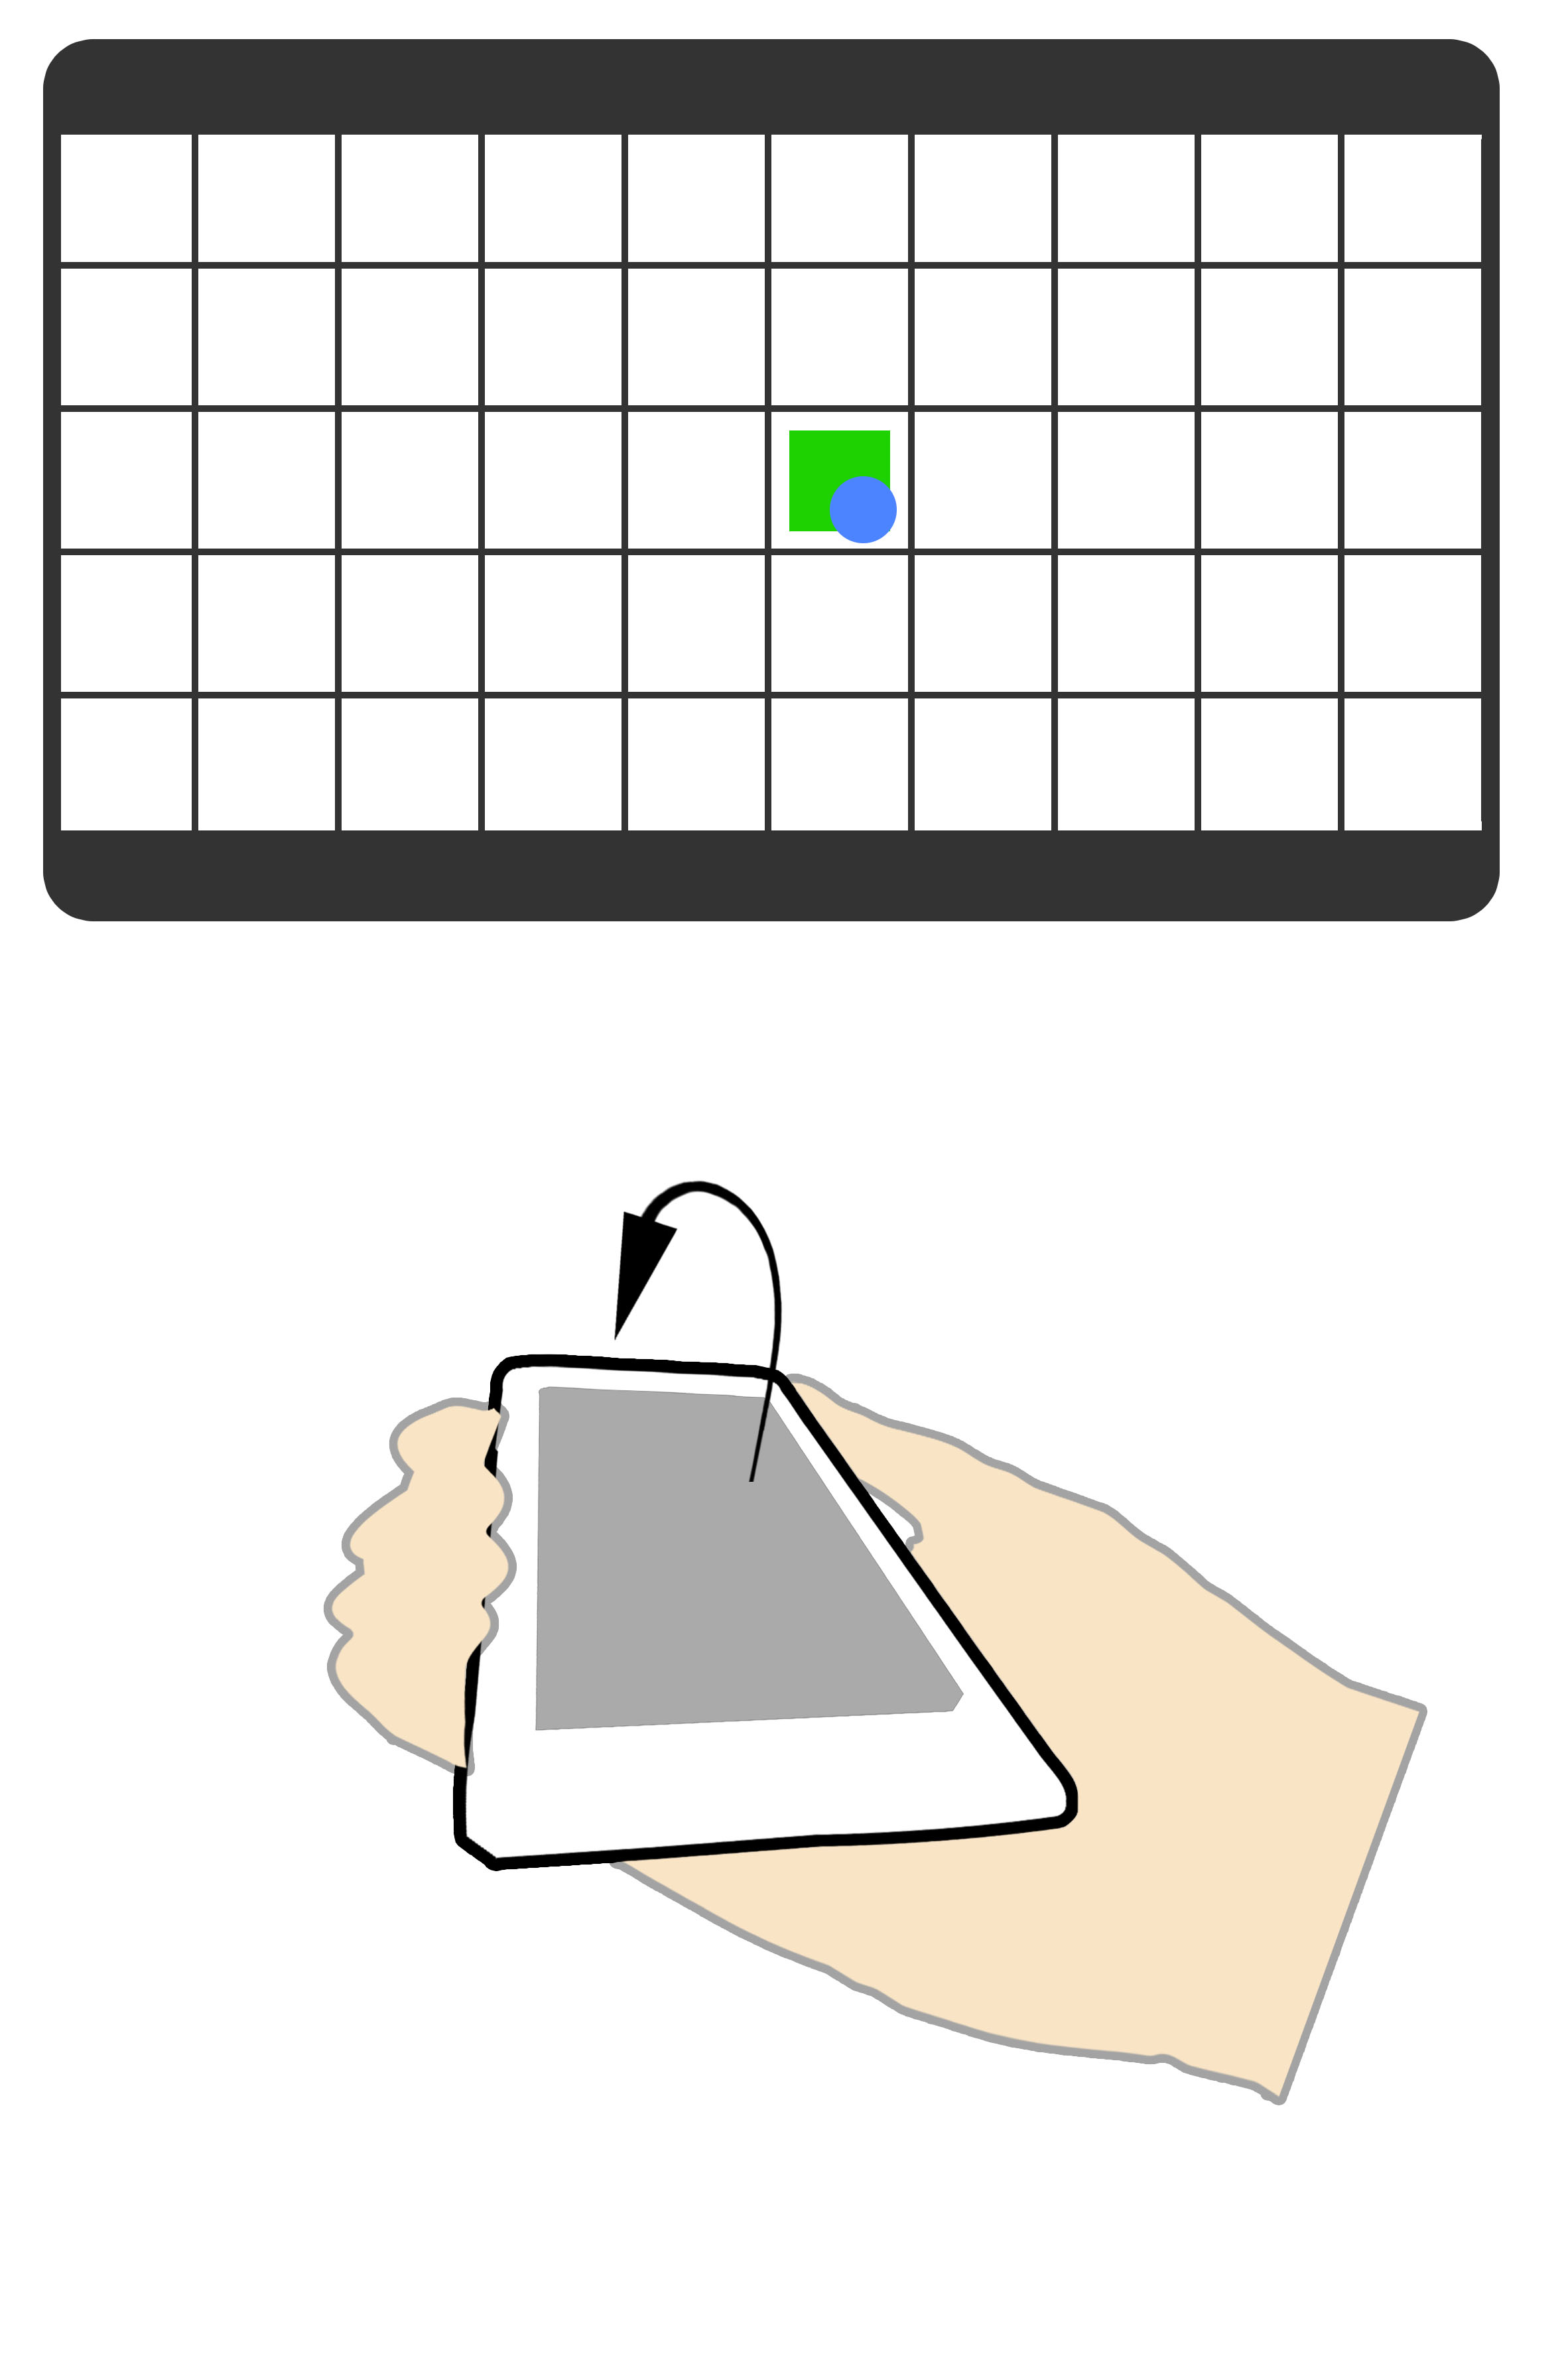
\includegraphics[width = 0.33\columnwidth]{images/techniques/tiltPush3.jpg}\label{fig:tiltPush3}}
	\caption{\push \grab technique}
	\label{fig:grabTechnique}
\end{figure}
% !TEX root = ../paper.tex
\section{Experiments} \label{sec:experiment}
% Intro
In order to compare  different techniques to each other we conducted an experiment in which each participant would perform the techniques in a controlled laboratory environment.
There are two studies to this experiment because after we finished the first experiment we realized that before we could say anything about accuracy in pixels we would have to design an experiment that required people to aim at a precise point and tell the participants to be as precise as they could.
Not having told our first 51 participants to aim and be precise we did the experiment again, adding a precise point to aim after for each target.
The first  experiment will be referred to as \target, and the second will be referred to as \accuracy.

\subsection{Implementation}
The four interaction techniques were implemented in a test application were the main goal was to correctly put shapes onto the screen from the smart phone or pull them away from the screen and put them on the phone.
The shapes would represent data, and two shapes(square and circle) were used in order to simulate the effect of choice of data. 

A grid system was implemented, were each target could be located in a particular grid cell.
The grid had two different sizes.
One was a large cell system, which had $5\times10$ cells, and each cell measured 61 pixels (7.3 cm) on each side.
The other was a small cell system, with $10\times20$ cells, each cell measuring 122 pixels (14.6 cm)  on each side. 

Shapes would appear in the cells, filling 80\% of it. 
These shapes would appear according to a predetermined series of locations, so that we could ensure that each target had an equal distribution of distances between them. 
For the user, the sequence would appear as random. 
These shapes would represent targets which the user had to hit.
A blue circle was used, as a cursor, to represent were the user is pointing on the screen.
This is where the user would ``hit'' whenever he performed an attempt with a given technique.

\begin{figure}[H]
	\subfloat[\push]{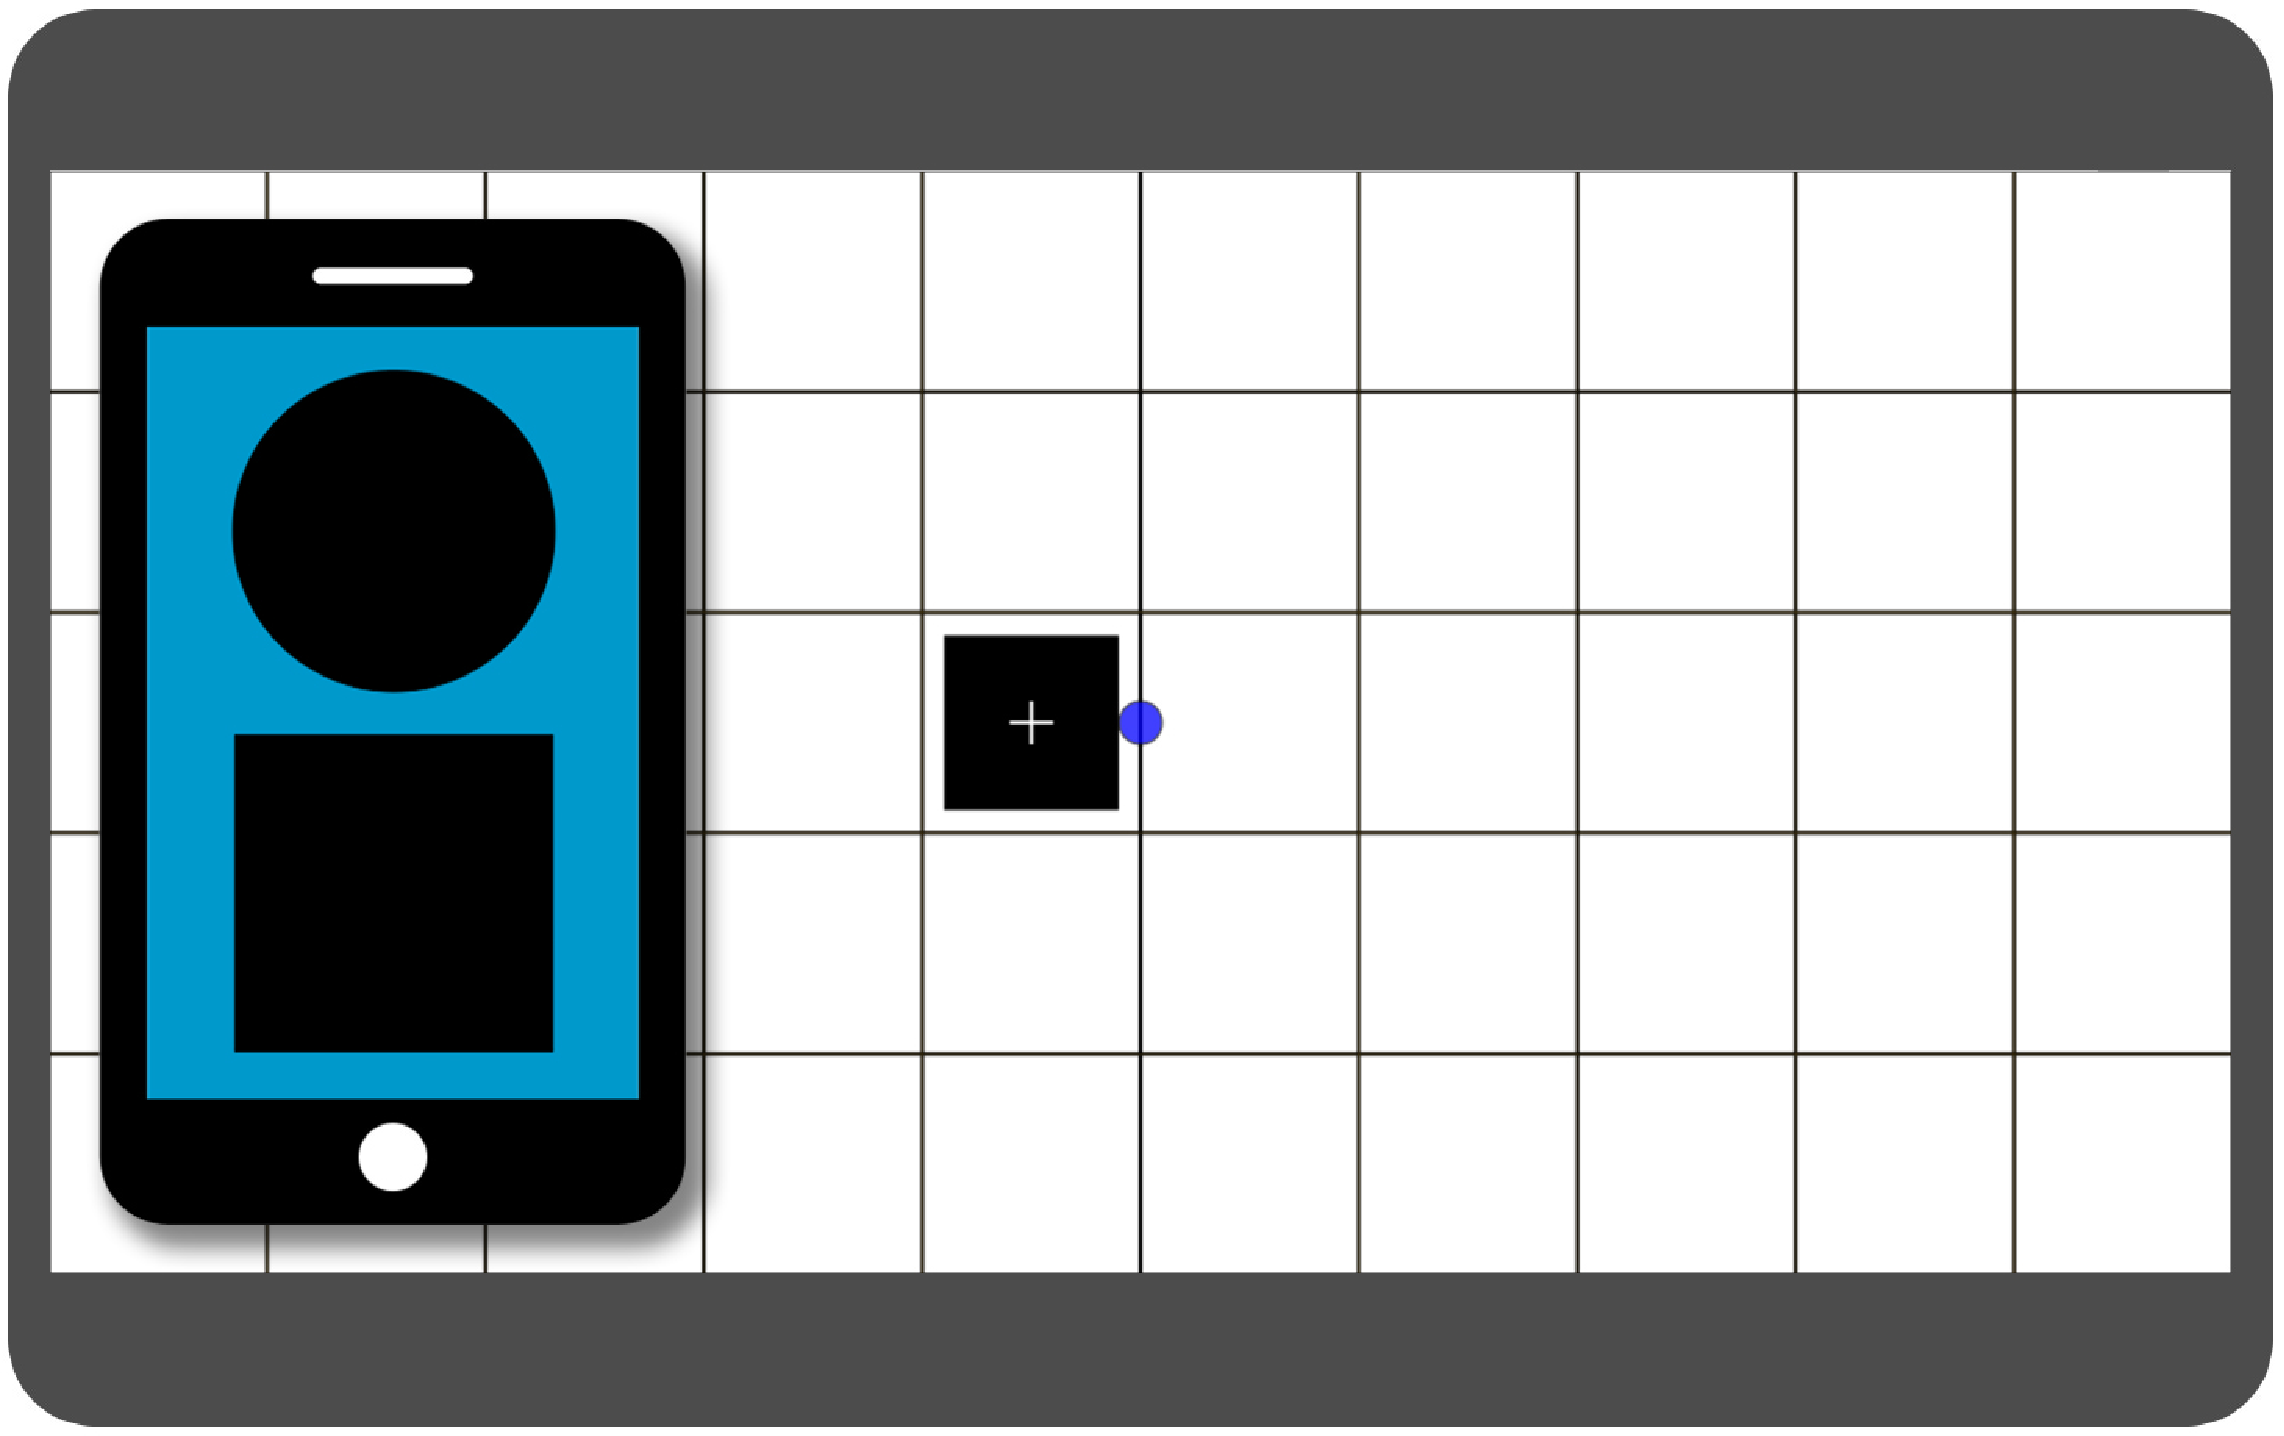
\includegraphics[width = 0.49\columnwidth]{images/pushScreen.pdf}\label{fig:pushScreen}}
	\hspace{0.01\columnwidth}
	\subfloat[\pull]{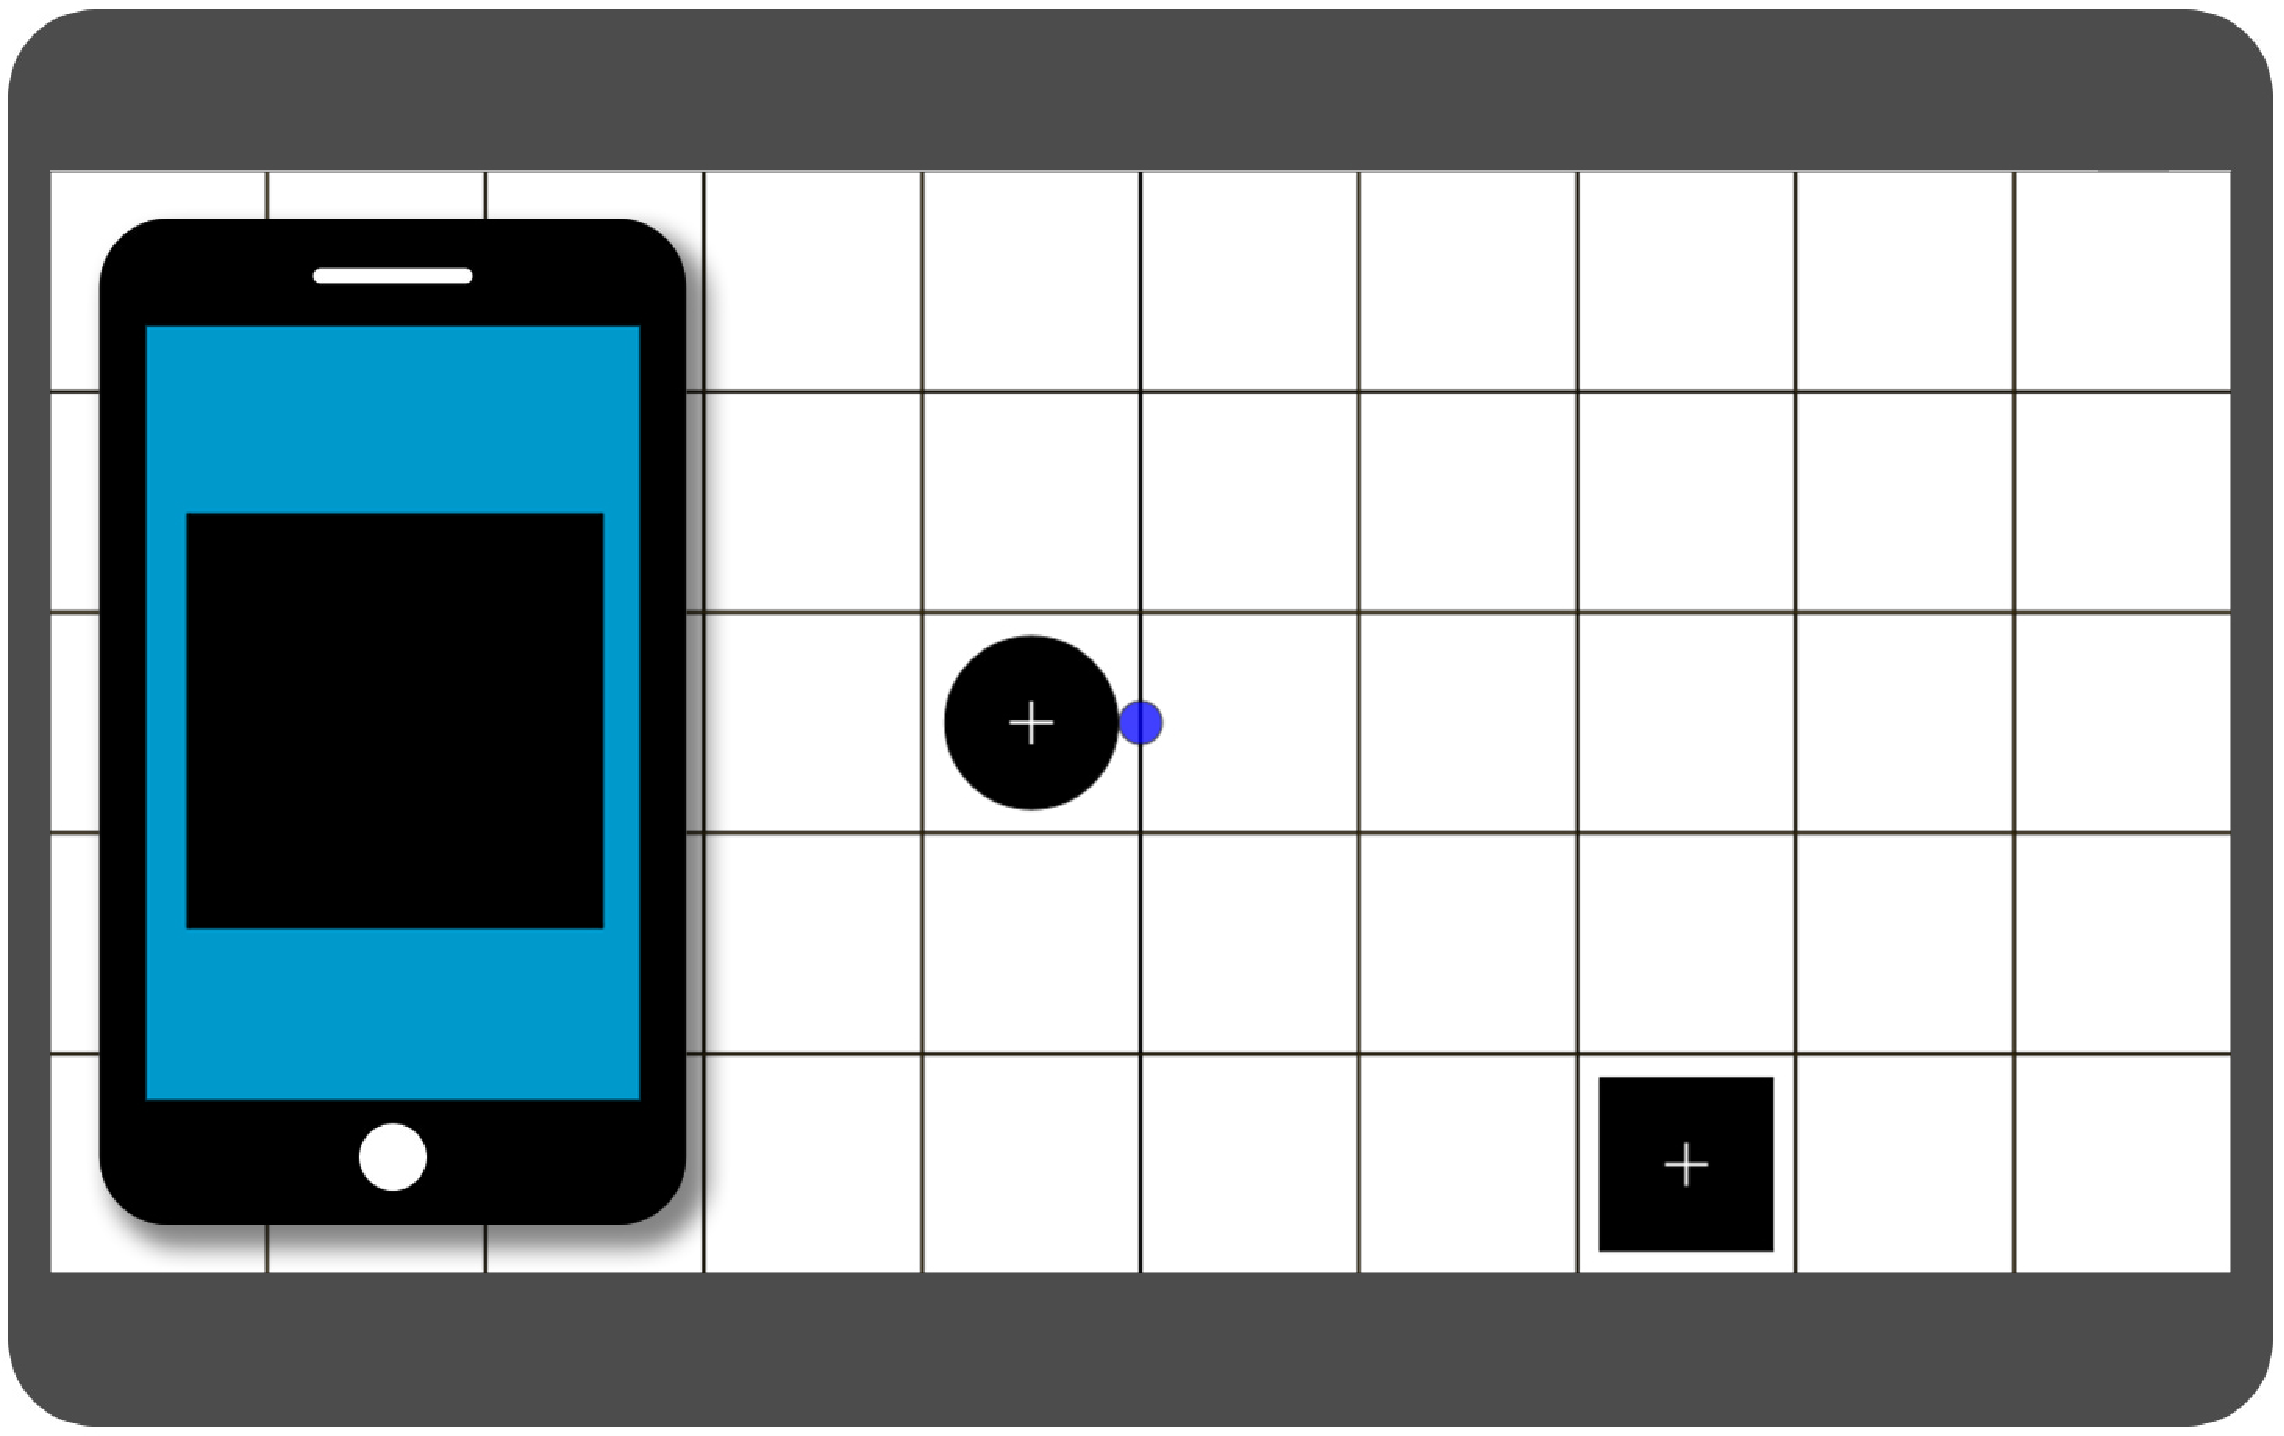
\includegraphics[width = 0.49\columnwidth]{images/pullScreen.pdf}\label{fig:pullScreen}}
	\caption{The screens on both the large display and the phone for the \accuracy.}
\end{figure}

During the \push phase of the experiment, users would be presented with one shape on the screen and two on the smartphone, as seen in \cref{fig:pushScreen}.
Here, the screen would tell the users what the correct shape was, and the user had to perform the technique by selecting the correct shape on the phone.
During the \pull phase of the experiment, users would be presented with two shapes on the large screen, and one shape on the smart phone.
Here, the phone would be telling users what the correct shape was and users would have to pull the correct shape from the large display. 
In the experiment, we conducted two separate studies, using the same implementation of techniques and experimental method. 

\subsubsection{Study One: Hit rate and time taken} 
During the \target, the circle used as a cursor was a solid blue color. 
There was also a bright yellow highlight in whichever cell the cursor was currently over.
This can be seen in \Cref{fig:target}.
This was for providing feedback to the user about whether or not he was hitting the correct cell. 

\subsubsection{Study Two: Precise distance from target}
During the \accuracy, we added a white cross to each target to provide a precise point for the users to aim at.
The circle cursor was also made opaque so that users could better see the cross, as well as removing the highlight so that users would not feel that hitting any part of the cell was acceptable.
This can be seen in \Cref{fig:accuracy}.
In study two, we explicitly asked users to be as precise as possible while performing each technique.

\begin{figure}[H]
\centering
\subfloat[]{\includegraphics[width = 0.13\columnwidth]{images/target.pdf}\label{fig:target}}
\hspace{0.05\columnwidth}
\subfloat[]{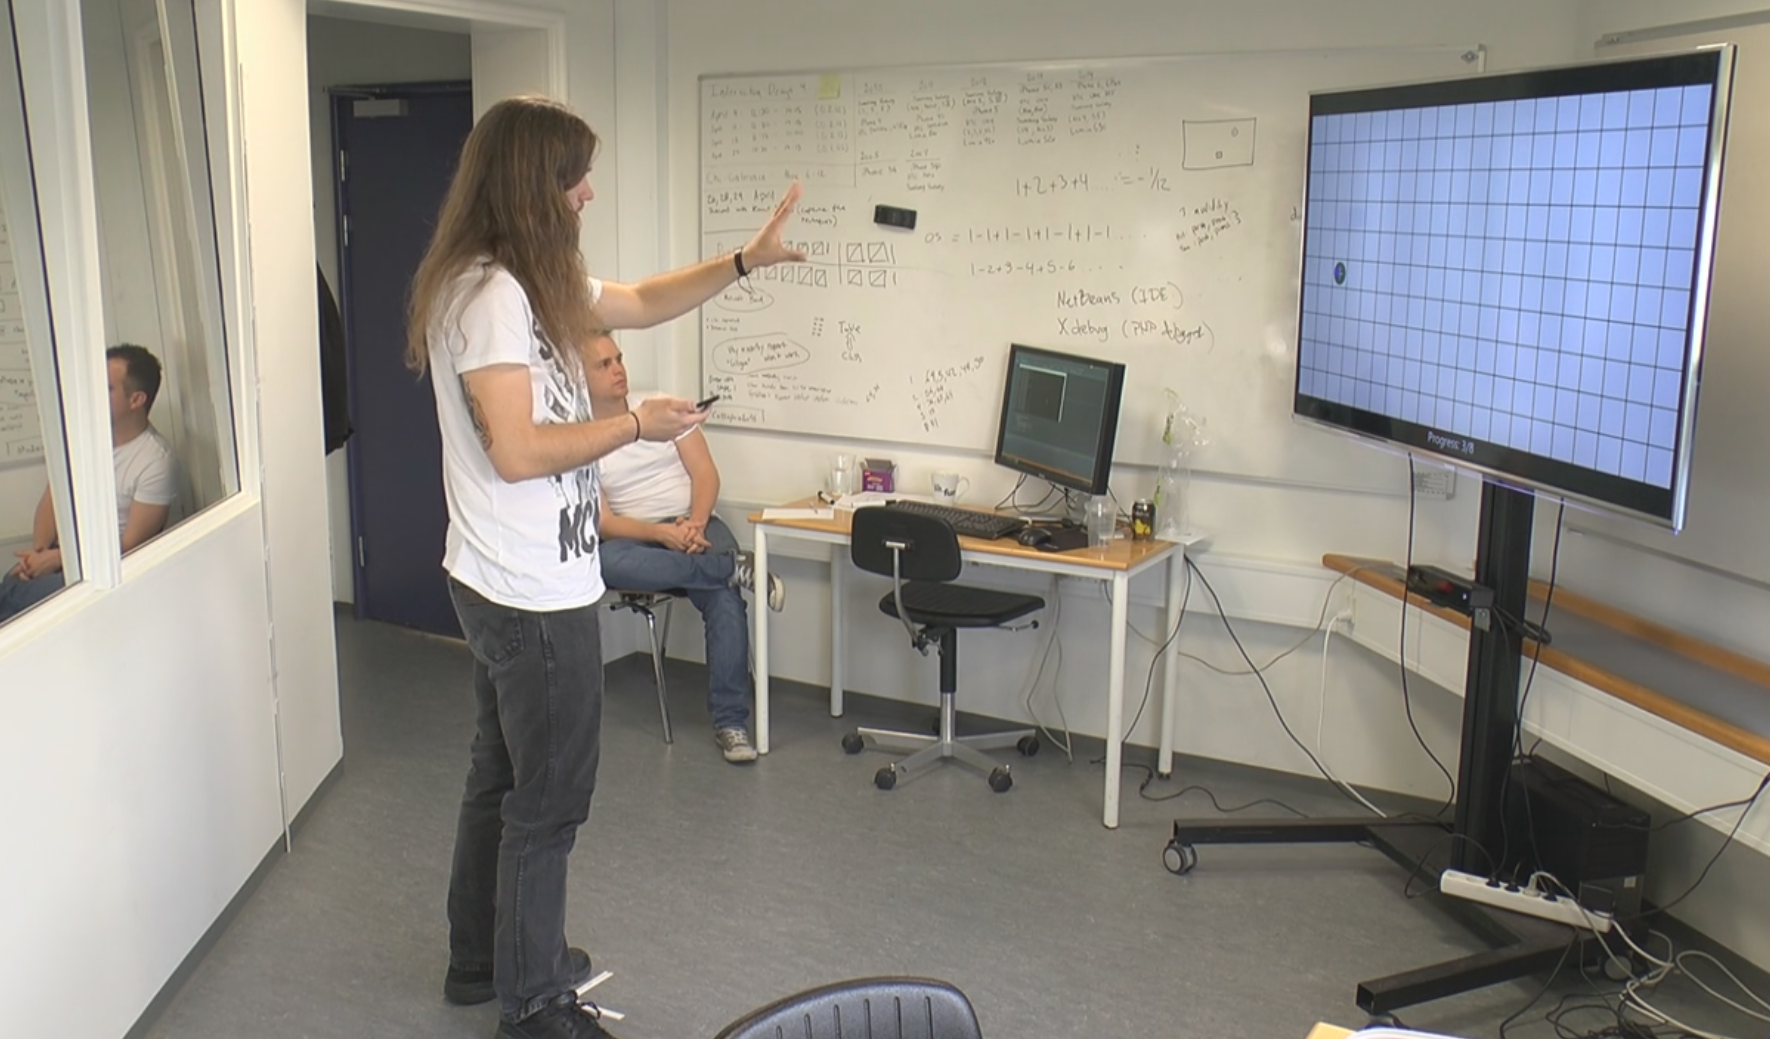
\includegraphics[width = 0.13\columnwidth]{images/accuracy.pdf}\label{fig:accuracy}}
\caption{\protect\subref{fig:target} The targets in the first part of the experiment. \protect\subref{fig:accuracy} The targets in the second part of the experiment.}
\end{figure}

\subsection{Experimental Setup} \label{sec:setup}
% The setup and the hardware used in the experiment
The experiment was conducted in laboratory setting where we setup a large 65'' screen (1920$\times$1080 pixels) and a smaller 42'' screen (1024$\times$768 pixels) as seen in \Cref{fig:setupPhoto}.
A Microsoft Kinect v2 was mounted below the large display (81 cm above the floor) and we marked the floor with a cross (200 cm from the Kinect) where participants were instructed to stand.
We chose 200 cm from the display because this is an optimal operating distance for the Kinect.
The height of the Kinect with regards to the floor was chosen through physical adjustment to get the optimal position for a person who is 180 cm tall (based on a estimation of average user height for Danish men (183 cm) and women(169cm)).
The phone we used in this experiment was a Samsung Galaxy S2 (4.3'' screen).
The setup is illustrated in \Cref{fig:setup}.

\begin{figure}[H]
\subfloat[]{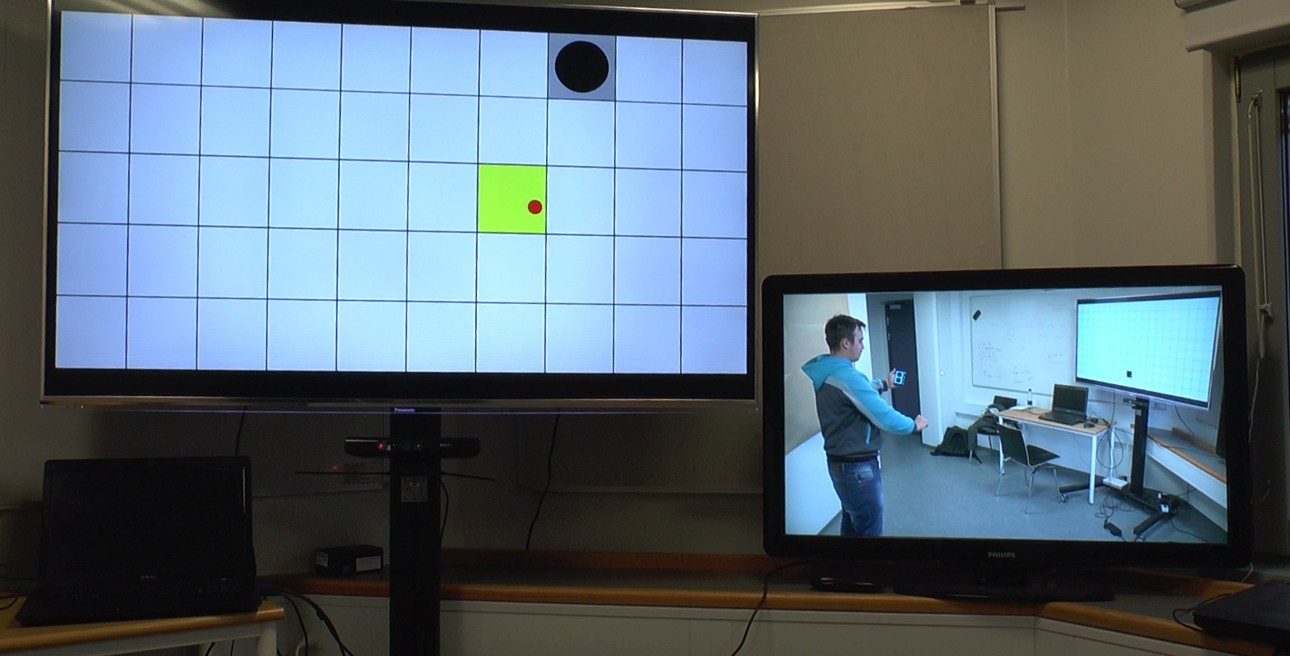
\includegraphics[width = 0.6\columnwidth]{images/setup.jpg}\label{fig:setupPhoto}}
\subfloat[]{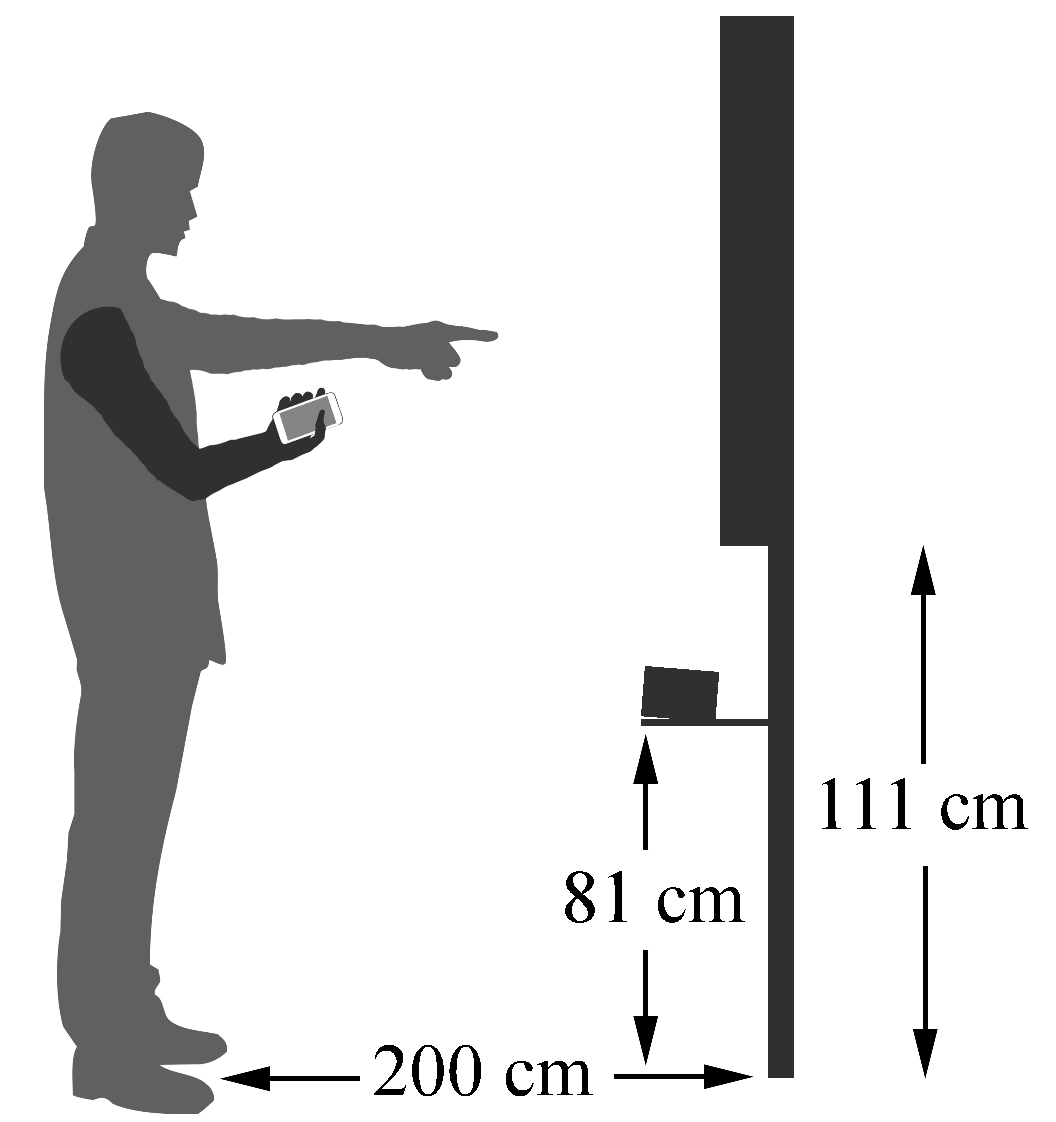
\includegraphics[width = 0.37\columnwidth]{images/setup.pdf}\label{fig:setup}}
\caption{\protect\subref{fig:setupPhoto} the setup in the usability lab. \protect\subref{fig:setup} illustrates the setup and distance between participant and screen, floor and Kinect, and floor and the bottom of the large display.}
\end{figure}

\subsubsection{Experimental Design} \label{}
% (explain practice targets, targets, grid, before procedure and task section)
% Also, explain sequences and the different distances between targets
A within-group design was used for the experiment and each participant used all 8 techniques once during the experiment.
We have 2 different target sizes (large, small) and 8 techniques (push = 4, pull = 4) as the independent variables.
For each technique there are a total of 18 targets and 3 practice targets at the beginning of each technique. 
Practice targets allow the participants to get familiar with the technique before we start collecting data for a technique.
The order in which the participants are presented with a technique is randomized to minimize the learning effect of each technique.
For both \target and \accuracy 51\% of the participants started with \push techniques and 49\% started with \pull techniques.
For \target 27\% of the participants started the test with \grab, 21\% with \swipe, 25\% with \throw, and 27\% with \tilt.
Similarly, for \accuracy 22\% of the participants started the test with \grab, 27\% with \swipe, 24\% with \throw, and 27\% with \tilt.
For \target the total amount of attempts collected were 2 target sizes $\times$ 8 techniques $\times$ 9 repetitions $\times$ 51 participants = 7344 attempts and for \accuracy the total is 2 target sizes $\times$ 8 techniques $\times$ 9 repetitions $\times$ 33 participants = 4752 attempts.

\subsubsection{Participants}
For the \target, 51 people took part. 
They ranged in age from 21 to 52 (M: 27,98) and were between 1.56m and 1.98m (M: 1,79m). 
15.7\% of participants were women, and 84.3\% were male.
All of the participants owned smartphones and had owned one for 2-12 years (M:5.9).

For the \accuracy, 33 people took part. They were between 20 and 55 years old (M: 23.18) and were between 1.56m and 2m tall (M: 1.77m).
30.3\% of the participants were female, while 69.7\% were male.
They had all owned smartphones for between 1 and 9 years (M: 5.5).

\subsubsection{Task \& Procedure} \label{sec:procedure}
The task and procedure were the same for both studies, with the additional instructions in \accuracy to be as precise as possible.
Before a participant starts the experiment, the general purpose of the study is explained to the participant and we inform them about what is going to happen.
Then a demonstration video of a technique is shown on the large screen and after watching the video it plays in a loop on the small screen.
The participant is then presented with the grid and one target after another will appear in the grid until the participant has attempted to hit all targets.
After completing one technique the remaining techniques follow with the same procedure as the first until all 8 techniques have been performed.
When a participant has done all the techniques we give them a short demographic questionnaire including age, height, gender, current phone, year of first smartphone, and if they have had prior experience with systems like the Nintendo Wii or the Microsoft Kinect.
The average time for completing the experiment per participant was 25$\pm$5 minutes. 
% !TEX root = ../paper.tex
%http://sphweb.bumc.bu.edu/otlt/MPH-Modules/BS/BS704_HypothesisTesting-ANOVA/BS704_HypothesisTesting-Anova_print.html
\section{Results}\label{sec:results}

Some data points needed to be removed from the experiments, in order to gain a clearer understanding of the data we just gathered. 


From the \target, we started with a total of 7344 attempts.
176 were removed because of system errors, were the system wrongly activated a technique attempt even though the user did not intend to do so.
Another 232 attempts were removed as outliers using the Outlier Labeling method described by Hoaglin and Iglewicz in Resistant Rules for Outlier Labeling \cite{Hoaglin:1987}.
This gave us a total of 6936 attempts for the \target.

From the \accuracy, we started with a total of 4752 attempts.
111 attempts were removed to system errors. 
Finally 130 attempts were removed with the same Outlier Labeling method used above.
This gave us a total of 4511 attempts for the \accuracy.

<<<<<<< HEAD
We then split up the data into two different data sets, the \push and \pull, in order to look at them independently. 

\Cref{tab:numberOfAttempts} shows the final number of attempts each technique had in the two different experiments

\begin{table}[H]
	\centering
	\textbf{Number of attempts}\\[4pt]
	\begin{adjustbox}{width=\columnwidth}
		\subfloat[\target]{
			\begin{tabular}{|c|c|c|c|c|}
				\hline
				\rowcolor[HTML]{9B9B9B} 
				& \textbf{Grab} & \textbf{Swipe} & \textbf{Throw} & \textbf{Tilt} \\ \hline
				Push & 830 & 896 & 889 & 862 \\ \hline
				Pull & 797 & 893 & 896 & 873 \\ \hline
			\end{tabular}
		}
		\subfloat[\accuracy] {
			\begin{tabular}{|c|c|c|c|c|}
				\hline
				\rowcolor[HTML]{9B9B9B} 
				& \textbf{Grab} & \textbf{Swipe} & \textbf{Throw} & \textbf{Tilt} \\ \hline
				Push & 551 & 583 & 566 & 575 \\ \hline
				Pull & 534 & 564 & 568 & 570 \\ \hline
			\end{tabular}
		}
	\end{adjustbox}
	\caption{Number of attempts for each technique in each experiment}
	\label{tab:numberOfAttempts}
\end{table}


\subsection{Success rate}
The results presented here will be based on the data collected during the \target. 
Here we will be presenting results relating to whether or not the user hit the target, which we will be referring to as effectiveness when discussing the results. 

To see whether or not each technique had an effect on the effectiveness of each attempt, we performed a Pearsons Chi-Square test on both data sets. 
For the \push techniques, $X(3)=121.950$, $p<0.000$, and for the \pull techniques we got $X(3)=438.473$, $p<0.000$. 
This means that both \push and \pull techniques had a significant effect on the effectiveness of each attempt. 
\Cref{tab:successRate} shows the success rate for each of the techniques. 

\begin{table}[H]
	\centering
	\textbf{Hit Success Means}\\[4pt]
	\begin{adjustbox}{width=\columnwidth}
		\begin{tabular}{|c|c|c|c|c|}
			\hline
			\rowcolor[HTML]{9B9B9B} 
			& \textbf{Grab} & \textbf{Swipe} & \textbf{Throw} & \textbf{Tilt} \\ \hline
			Push & 95.9\% & 95.8\% & 92.6\% & 83.3\% \\ \hline
			Pull & 94\% & 97.5\% & 96.4\% & 71.5\% \\ \hline
		\end{tabular}
	\end{adjustbox}
	\caption{Success rate for each technique}
	\label{tab:successRate}
\end{table}

\subsection{Time taken}
This section will be presenting results based on the \target.
Here, we will be presenting the results in regards to how long each user took in performing each technique. 
When discussing these results, we will be referring to them as a techniques efficiency.

We performed a linear mixed effects model analysis on the data to see whether or not each technique had a significant effect on the efficiency of each attempt. 

\subsection{Distance from target}
The data that was used to measure the distance from the target was based on the \accuracy experiment.
Here we will present the results in regards to how far away from the center of the target (in pixels) each user was when performing the technique. 
This will be referred as a a techniques accuracy when we discuss the results presented in this section. 

We performed another linear mixed effects model analysis on the data to see if each technique had a significant effect on the accuracy of each attempt. 



% !TEX root = ../paper.tex
\section{Discussion}\label{sec:discussion}
% !TEX root = ../report.tex
\section*{Concluding Remarks} \label{sec:conclusion}
\addcontentsline{toc}{section}{Concluding Remarks}

This thesis deals with the theme of cross-device interaction between mobile devices and large displays. 
We approached this theme by finding and implementing 8 different interaction techniques and then performing a comparative study between them.

One of the ideas behind this thesis was to see if we could find any attributes to these techniques that made them successful in regards to accuracy and efficiency.
We initially believed that the some of the important attributes to the success of a technique would be whether or not the phone was in motion during the technique and the amount of hands used to perform the given technique.

Our results did show that there might be some association between the amount of hands and the accuracy and efficiency of each technique. 
There seems to be some indication that one handed techniques are faster to perform that two handed, but that two handed techniques are more accurate.
These are only indications though and in order to more conclusively say that this is indeed the case, more research must be conducted with these specific attributes in mind.  

A much more important attribute though came up and that was the ability to hold the cursor still while performing the technique. 
The two most successful techniques, \emph{Swipe} and \emph{Throw} both had that in common. 
Users where capable of keeping the cursor still while activating and performing the technique.
The other two techniques, \emph{Tilt} and \emph{Grab}, both movements on the cursor pointing hand, causing the cursor to move during activation instead of keeping it stable. 

In the future, we would like to extend our research by examining more closely the relationship between amount of hands and the efficiency and accuracy of each technique. 
This could be done by implementing different techniques were the focus is much more on the amount of hands and the role of each hand while performing the given technique.
Having techniques were the sole role of one of the hands is for aiming, like \emph{Throw}, and others were each hand has some gesture it has to perform in order to activate the technique, such as \emph{Grab}.
A research like this could lead to a much more clear understanding of how the amount of hands affects the performance of a interaction technique.
% !TEX root = ../paper.tex
\section{Future Research} \label{sec:futureresearch}
Future work could attempt to answer the question of whether or not one handed or two handed techniques are more efficient and accurate.
Our focus has been purely on a quantitative understanding of interaction techniques: time taken, success and distance in pixels.
There are many more facets to interaction techniques than this. 
Future research could do a qualitative study on users opinion of the different techniques. 
One could also attempt to utilize each technique in a public setting since large public display are becoming more and more prevalent. 
This could lead to a better understanding of the social implications of using such techniques in a public setting.
Finally, we could explore the learning curves of each technique, to better understand the use context for each of these interaction techniques. 
% !TEX root = ../paper.tex
\section{Acknowledgments}\label{sec:acknowledgment}


%\subsection{References and Citations}
%
%Use a numbered list of references at the end of the article, ordered
%alphabetically by last name of first author, and referenced by numbers
%in
%brackets~\cite{acm_categories,ethics,Klemmer:2002:WSC:503376.503378}.
%Your references should be published materials accessible to the
%public. Internal technical reports may be cited only if they are
%easily accessible (i.e., you provide the address for obtaining the
%report within your citation) and may be obtained by any reader for a
%nominal fee. Proprietary information may not be cited. Private
%communications should be acknowledged in the main text, not referenced
%(e.g., ``[Borriello, personal communication]'').
%
%References should be in ACM citation format:
%\url{http://acm.org/publications/submissions/latex_style}. This
%includes citations to internet
%resources~\cite{acm_categories,cavender:writing,CHINOSAUR:venue,psy:gangnam}
%according to ACM format, although it is often appropriate to include
%URLs directly in the text, as above.


% Use a numbered list of references at the end of the article, ordered
% alphabetically by first author, and referenced by numbers in
% brackets~\cite{ethics, Klemmer:2002:WSC:503376.503378,
%   Mather:2000:MUT, Zellweger:2001:FAO:504216.504224}. For papers from
% conference proceedings, include the title of the paper and an
% abbreviated name of the conference (e.g., for Interact 2003
% proceedings, use \textit{Proc. Interact 2003}). Do not include the
% location of the conference or the exact date; do include the page
% numbers if available. See the examples of citations at the end of this
% document. Within this template file, use the \texttt{References} style
% for the text of your citation.

% Your references should be published materials accessible to the
% public.  Internal technical reports may be cited only if they are
% easily accessible (i.e., you provide the address for obtaining the
% report within your citation) and may be obtained by any reader for a
% nominal fee.  Proprietary information may not be cited. Private
% communications should be acknowledged in the main text, not referenced
% (e.g., ``[Robertson, personal communication]'').

% Balancing columns in a ref list is a bit of a pain because you
% either use a hack like flushend or balance, or manually insert
% a column break.  http://www.tex.ac.uk/cgi-bin/texfaq2html?label=balance
% multicols doesn't work because we're already in two-column mode,
% and flushend isn't awesome, so I choose balance.  See this
% for more info: http://cs.brown.edu/system/software/latex/doc/balance.pdf
%
% Note that in a perfect world balance wants to be in the first
% column of the last page.
%
% If balance doesn't work for you, you can remove that and
% hard-code a column break into the bbl file right before you
% submit:
%
% http://stackoverflow.com/questions/2149854/how-to-manually-equalize-columns-
% in-an-ieee-paper-if-using-bibtex
%
% Or, just remove \balance and give up on balancing the last page.
%
\balance{}

% REFERENCES FORMAT
% References must be the same font size as other body text.
\bibliographystyle{SIGCHI-Reference-Format}
\bibliography{Paper}

\end{document}

%%% Local Variables:
%%% mode: latex
%%% TeX-master: t
%%% End:
